% Hardware-in-the-loop evolutionary search for FHE parameters on Apple Silicon
%
% Build:  latexmk -pdf main.tex
% Clean:  latexmk -C
%
% body.tex is generated from ../PAPER_ABSTRACT.md by scripts/build-paper.sh.
% Do not edit body.tex directly; edit the Markdown source and regenerate.

\documentclass[11pt,a4paper]{article}

% --- encoding and fonts ---------------------------------------------------
% The Markdown source contains characters pdfLaTeX cannot typeset directly:
% U+2212 MINUS SIGN, subscript digits in log_2(q), and a bare sigma in prose.
% Under XeLaTeX these are handled natively by a Unicode font; under pdfLaTeX
% they are declared explicitly below. Build with either.
% Build with pdfLaTeX. A XeLaTeX path was attempted and removed: it needs
% fontspec font resolution that fails on hosts carrying only the
% TeX-distribution copy of Latin Modern, and it buys nothing here because the
% declarations below cover every non-ASCII character the source actually uses.
\usepackage{iftex}
\ifPDFTeX
  \usepackage[T1]{fontenc}
  \usepackage[utf8]{inputenc}
  \usepackage{lmodern}
  \usepackage{textcomp}
  % Characters pandoc passes through from the Markdown source.
  \DeclareUnicodeCharacter{2212}{\textminus}
  \DeclareUnicodeCharacter{2080}{\ensuremath{_0}}
  \DeclareUnicodeCharacter{2081}{\ensuremath{_1}}
  \DeclareUnicodeCharacter{2082}{\ensuremath{_2}}
  \DeclareUnicodeCharacter{03C3}{\ensuremath{\sigma}}
  \DeclareUnicodeCharacter{03C8}{\ensuremath{\psi}}
  \DeclareUnicodeCharacter{03C9}{\ensuremath{\omega}}
  \DeclareUnicodeCharacter{2248}{\ensuremath{\approx}}
  \DeclareUnicodeCharacter{2261}{\ensuremath{\equiv}}
  \DeclareUnicodeCharacter{2265}{\ensuremath{\geq}}
  \DeclareUnicodeCharacter{2264}{\ensuremath{\leq}}
  \DeclareUnicodeCharacter{00D7}{\ensuremath{\times}}
  \DeclareUnicodeCharacter{00B5}{\textmu}
  \DeclareUnicodeCharacter{00E8}{\`e}
  \DeclareUnicodeCharacter{2192}{\ensuremath{\rightarrow}}
  \DeclareUnicodeCharacter{2713}{\ensuremath{\checkmark}}
  \DeclareUnicodeCharacter{2717}{\ensuremath{\times}}
\else
  % No \setmainfont: fontspec defaults to Latin Modern, which is what the
  % pdfLaTeX branch uses via lmodern. Naming it explicitly as a system font
  % fails on hosts where only the TeX-distribution version is installed
  % (the "missing fonts" failure mode under XeLaTeX). Prefer pdfLaTeX.
  \usepackage{fontspec}
  \usepackage{unicode-math}
\fi
\usepackage[english]{babel}

% --- mathematics ----------------------------------------------------------
\usepackage{amsmath}
\usepackage{amssymb}
\usepackage{amsthm}

% --- tables ---------------------------------------------------------------
% Pandoc emits longtable for Markdown pipe tables, which needs both of these.
\usepackage{longtable}
\usepackage{booktabs}
\usepackage{array}
\usepackage{calc}

% --- layout ---------------------------------------------------------------
\usepackage[margin=1in]{geometry}
\usepackage{microtype}
\setlength{\parskip}{0.4em}

% --- figures and links ----------------------------------------------------
\usepackage{graphicx}
\usepackage{xcolor}
\usepackage[
  colorlinks=true,
  linkcolor=black,
  citecolor=black,
  urlcolor=blue!60!black,
  breaklinks=true
]{hyperref}
\usepackage{url}

% --- code and verbatim ----------------------------------------------------
% Pandoc wraps fenced code blocks in Shaded/Highlighting when a highlighting
% style is active; providing these keeps the document compiling if it does.
\usepackage{fancyvrb}
\usepackage{framed}
\providecommand{\tightlist}{%
  \setlength{\itemsep}{0pt}\setlength{\parskip}{0pt}}
\providecommand{\pandocbounded}[1]{#1}

% Pandoc emits \def\LTcaptype{none} for a longtable with no caption, and
% longtable then tries to step a counter named `none'. Define it so the
% suppression works instead of erroring once per table.
\newcounter{none}

% --- metadata -------------------------------------------------------------
% Title matches the Markdown H1 in ../PAPER_ABSTRACT.md (the source of truth).
\title{Hardware-Aware FHE Parameter Discovery via\\
       Multi-Objective Evolutionary Optimization\\
       on Apple Silicon}
\author{Jessica Mulein\\\small Digital Defiance}
\date{\today}

\begin{document}
\maketitle

\begin{abstract}

Fully Homomorphic Encryption parameter selection remains dominated by conservative theoretical bounds --- notably the HE Standard 2018 --- which guarantee security but ignore the performance characteristics of specific hardware platforms. We present a hardware-in-the-loop evolutionary methodology that searches FHE parameter configurations against three objectives: measured NTT computation latency, estimated lattice security level, and noise growth budget.

Our system employs NSGA-II (Non-dominated Sorting Genetic Algorithm II) with populations stratified by polynomial degree (\(N \in \{1024, 2048, 4096, 8192, 16384\}\)). Each candidate parameter set is evaluated through actual Number Theoretic Transform execution on Apple M4 Max silicon via a Rust FFI layer with NEON SIMD acceleration, providing ground-truth latency measurements rather than theoretical complexity estimates. A security sieve applies a 128-bit minimum security floor using a calibrated lattice-reduction cost heuristic before any candidate enters the benchmark pipeline.

The contribution is twofold: a reusable methodology for hardware-in-the-loop multi-objective parameter search, and a measured characterisation of NTT cost on M4 Max across five polynomial degree tiers. The principal empirical finding is negative and practically useful: at FHE-relevant scales, NTT latency is insensitive to which NTT-friendly modulus is chosen at fixed \(N\). Within a tier, the best measured latency per modulus varies by 3.7--9.4\% across all moduli present on the frontier --- with no post-hoc filtering --- whereas each doubling of \(N\) costs a factor of approximately 2.15×. The insensitivity is corroborated from the optimiser's side: across all five tiers, 10,000 generations of NSGA-II move the best measured latency by between −0.3\% and +0.5\%, so the latency optimum is already present in the initial random population and the search contributes frontier breadth rather than depth. A practitioner needing only the fastest configuration at a given \(N\) can therefore obtain it by sampling the modulus pool, and the evolutionary machinery earns its cost only when the full three-objective trade-off surface is wanted. Consequently, modulus selection can be driven by security and noise-budget requirements without incurring a latency penalty, and hardware-aware optimisation matters at the granularity of \(N\) rather than within a tier. Measured cross-tier scaling reproduces \(O(N \log N)\) to within 3.5\%. On the tuned Montgomery path the insensitivity is stronger still: negacyclic NTT latency is invariant not only across moduli within a tier but across modulus \emph{width}: it is essentially unchanged between a 27-bit and a 60-bit modulus at every degree measured (7.98 against 7.92 µs at \(N = 1024\), 174.75 against 174.72 µs at \(N = 16384\)). A validated Metal compute-shader batch negacyclic NTT, gated behind a negacyclic convolution identity as well as exact coefficient-level agreement with the CPU reference, delivers 4.6×--5.9× over the fastest measured CPU NTT path once the batch is large enough to amortise dispatch cost. We also report a methodological result with implications beyond this study: round-trip verification cannot validate an NTT, because a forward/inverse pair recovers its input for any nonzero twiddle table, and four defective transforms in this codebase passed it. The methodology generalises to any platform where NTT benchmarking is feasible, enabling per-hardware parameter catalogs for practical FHE deployment.

\end{abstract}

\textbf{Keywords:} Fully Homomorphic Encryption, Multi-Objective Optimization, NSGA-II, Number Theoretic Transform, Apple Silicon, Pareto Optimization, Lattice Cryptography

\section{Introduction}\label{introduction}

Fully Homomorphic Encryption (FHE) enables computation on encrypted data without decryption, offering a transformative approach to privacy-preserving computation in cloud environments, multi-party analytics, and outsourced machine learning inference. Despite significant theoretical advances since Gentry's foundational construction [1], practical deployment remains limited by computational overhead --- FHE operations are typically orders of magnitude slower than their plaintext equivalents. Parameter selection is one of the levers available for reducing that overhead.

The core challenge lies in the interdependence of FHE parameters. The polynomial degree \(N\), ciphertext modulus \(q\), noise standard deviation \(\sigma\), and gadget decomposition base \(B_g\) collectively determine three competing properties: cryptographic security (resistance to lattice attacks), computational performance (dominated by polynomial multiplication via the Number Theoretic Transform), and noise budget (the depth of homomorphic computation before decryption failure). Increasing \(N\) improves security but increases NTT cost as \(O(N \log N)\). Increasing \(q\) expands the noise budget but weakens security. The resulting tradeoff space is high-dimensional, discrete, and highly constrained.

Current practice relies on parameter tables derived from the Homomorphic Encryption Standard [2], which provides maximum modulus sizes for each polynomial degree at fixed security levels. These tables are inherently conservative: they target worst-case lattice attack costs, assume idealised computation, and are platform-agnostic. They also give no guidance on where to sit within the allowed range for a particular machine.

We address this gap with an evolutionary multi-objective optimisation system that searches FHE parameter configurations through hardware-in-the-loop benchmarking. The system uses NSGA-II [3] with populations stratified by polynomial degree, evaluating each candidate through actual NTT execution on Apple M4 Max silicon. A lattice security sieve applies a 128-bit minimum security floor. The result is a per-hardware frontier over latency, estimated security margin, and noise budget, together with a direct measurement of how NTT cost responds to each parameter.

The contributions of this paper are: (1) a three-layer architecture combining Node.js orchestration, security estimation, and Rust execution with NEON SIMD acceleration for hardware-in-the-loop FHE parameter evaluation; (2) a genome representation and mutation strategy that maintains NTT-friendly prime constraints throughout evolution; (3) a measured characterisation of NTT cost on Apple M4 Max, including the negative result that latency is essentially invariant in the choice of NTT-friendly modulus at fixed \(N\) while cross-tier scaling tracks \(O(N \log N)\) closely; (4) an explicit account of the validity threats that this class of study is exposed to, including objective degeneracy and estimator fidelity (Section 6.7); and (5) a demonstration that round-trip verification cannot validate an NTT, with four defective transforms in this codebase that passed it, two of them in code paths that produced published measurements (Section 6.6).

The remainder of this paper is organized as follows. Section 2 reviews background on FHE parameters, the HE Standard, multi-objective optimization, and hardware-aware cryptographic tuning. Section 3 presents the system design. Section 4 details implementation specifics. Section 5 describes the experimental setup. Section 6 presents results. Section 7 discusses implications and limitations. Section 8 concludes.

\section{Background and Related Work}\label{background-and-related-work}

\subsection{Fully Homomorphic Encryption Parameters}\label{fully-homomorphic-encryption-parameters}

Modern FHE schemes --- including TFHE [4], BFV, and CKKS --- are built on the hardness of the Ring Learning With Errors (RLWE) problem [9]. Computations are performed over polynomial rings \(\mathbb{Z}_q[X]/(X^N + 1)\), where \(N\) is the polynomial degree (a power of two) and \(q\) is the ciphertext modulus. The noise standard deviation \(\sigma\) controls the magnitude of error terms added during encryption to mask the plaintext, while the gadget decomposition base \(B_g\) determines the granularity of key switching and bootstrapping operations.

These parameters interact in complex ways. The polynomial degree \(N\) determines the lattice dimension and thus the security level against known lattice reduction attacks (BKZ, sieving). The modulus \(q\) controls the ``space'' available for noise growth during computation --- larger \(q\) permits more operations before noise overwhelms the message, but weakens security by making the LWE distinguishing problem easier. The noise \(\sigma\) must be large enough to provide statistical security guarantees (the HE Standard and common practice assume \(\sigma \geq 3.2\)), yet small enough to preserve noise budget for computation.

The computational bottleneck in all these schemes is polynomial multiplication, which is performed via the Number Theoretic Transform (NTT) --- the finite field analog of the Fast Fourier Transform. NTT transforms an \(N\)-coefficient polynomial from coefficient representation to evaluation representation in \(O(N \log N)\) operations modulo \(q\), enabling element-wise multiplication followed by an inverse NTT. Because FHE operates in the negacyclic ring \(\mathbb{Z}_q[X]/(X^N + 1)\), the transform requires a primitive \(2N\)-th root of unity in \(\mathbb{Z}_q\), which holds if and only if \(q \equiv 1 \pmod{2N}\). The weaker condition \(q \equiv 1 \pmod{N}\) suffices only for the cyclic transform over \(X^N - 1\). The evolutionary search, the reduction-strategy measurements of Section 6.4, and the GPU measurements of Section 6.5 all enforce the stronger negacyclic condition \(q \equiv 1 \pmod{2N}\). This ``NTT-friendly prime'' constraint significantly restricts the feasible parameter space.

\subsection{The Homomorphic Encryption Standard}\label{the-homomorphic-encryption-standard}

The Homomorphic Encryption Standard [2], published in 2018 by Albrecht et al., provides recommended parameter ranges for lattice-based cryptographic schemes targeting specific security levels. For 128-bit security (resistance equivalent to \(2^{128}\) operations for the best known attack), the standard specifies maximum modulus sizes: \(\log_2(q) \leq 27\) for \(N = 1024\), \(\log_2(q) \leq 54\) for \(N = 2048\), \(\log_2(q) \leq 109\) for \(N = 4096\), \(\log_2(q) \leq 218\) for \(N = 8192\), and \(\log_2(q) \leq 438\) for \(N = 16384\).

These bounds are derived from lattice reduction cost models --- primarily the Core-SVP methodology --- which estimate the number of operations required to solve the shortest vector problem in a lattice of dimension \(N\) with modulus-to-noise ratio \(q/\sigma\). The standard intentionally errs on the side of caution: it assumes the most optimistic attack strategies, provides no guidance on choosing within the allowed range, and is entirely platform-agnostic. This conservatism, while appropriate for a security standard, leaves practitioners without platform-specific guidance.

\subsection{Multi-Objective Evolutionary Optimization}\label{multi-objective-evolutionary-optimization}

Multi-objective optimization problems involve simultaneously optimizing two or more conflicting objectives. Unlike single-objective optimization, there is generally no single solution that optimizes all objectives simultaneously. Instead, the goal is to find the Pareto front --- the set of solutions where no objective can be improved without degrading another.

NSGA-II (Non-dominated Sorting Genetic Algorithm II) [3] is the canonical algorithm for multi-objective evolutionary optimization. It operates on a population of candidate solutions, ranking them by Pareto dominance: solution \(A\) dominates \(B\) if \(A\) is at least as good as \(B\) on all objectives and strictly better on at least one. The algorithm assigns each solution a rank based on its dominance front (rank 1 = non-dominated, rank 2 = dominated only by rank 1, etc.) and uses crowding distance --- a measure of isolation in objective space --- as a secondary selection criterion to maintain diversity along the frontier.

Assessing the quality of an approximated front is itself a research area; Zitzler et al.~[14] survey the available indicators and their failure modes, including the observation that front cardinality alone is a weak proxy for approximation quality. Section 6.2 reports front size over time because it is what the run recorded, and Section 6.7 notes the limits of that measure.

Evolutionary approaches are well-suited to FHE parameter discovery for several reasons: the search space is discrete and highly constrained (NTT-friendly prime requirement), the objective functions are expensive to evaluate (requiring actual hardware benchmarking), and no gradient is available through the measurement.

\subsection{Hardware-Aware Cryptographic Optimization}\label{hardware-aware-cryptographic-optimization}

Prior work on hardware-specific cryptographic optimization has focused primarily on implementation efficiency rather than parameter selection. Longa and Naehrig [8] demonstrated NTT speedups through algorithmic improvements (lazy reduction, merged operations). The NTT has also been implemented on GPUs, FPGAs and ASICs, achieving throughput improvements through parallelism. These works optimize the implementation for fixed parameters rather than optimizing parameters for a fixed implementation.

Apple Silicon presents a distinctive hardware profile for lattice cryptography. The unified memory architecture eliminates the PCIe bottleneck between CPU and accelerator memory. The NEON SIMD unit provides 128-bit vector operations with two 64-bit lanes. The wide out-of-order execution cores (12 performance cores on M4 Max [10]) provide high instruction-level parallelism for independent butterfly operations. Vendor-reported memory bandwidth for the 16-core-CPU / 40-core-GPU M4 Max configuration used here is 546 GB/s [10].

Two additional acceleration paths are frequently cited for Apple Silicon and warrant caution. The Apple Matrix coprocessor (AMX) is undocumented and its instruction encoding is known only through reverse engineering; the Scalable Matrix Extension (SME) is architecturally specified but its availability and dispatch behaviour vary. A third-party library exposing a backend \emph{labelled} ``AMX'' does not by itself establish that AMX instructions were issued for a given call. We observed a concrete inconsistency of this kind: the Node addon's \texttt{detectHardware()} reported AMX as unavailable in sessions where the accompanying C++ harness reported it as available. We therefore make no claims about AMX or SME behaviour in this paper, and Section 6.4 restricts itself to reduction strategies we could measure and attribute unambiguously.

We are not aware of prior work applying \emph{evolutionary} search with hardware-in-the-loop NTT measurement to FHE parameter selection. Automated parameter selection has been explored in the FHE compiler literature, where the objective is typically circuit-specific noise budgeting rather than hardware-measured latency.

\section{System Design}\label{system-design}

\subsection{Architecture Overview}\label{architecture-overview}

The system comprises three distinct layers separated by well-defined interfaces. The orchestration layer (Node.js/TypeScript) manages population lifecycle, evolutionary selection, and result serialization. The security layer (TypeScript) implements the lattice security estimator and acts as a filter (``guillotine'') preventing insecure configurations from consuming benchmark resources. The execution layer (Rust with NEON intrinsics) implements the NTT benchmark sandbox and provides ground-truth latency measurements.

The FFI boundary between Node.js and Rust is designed for zero-overhead batch processing. Parameter genomes are packed into flat \texttt{Uint32Array} buffers (\texttt{{[}N₀,\ q₀,\ σ₀,\ Bg₀,\ N₁,\ q₁,\ σ₁,\ Bg₁,\ ...{]}}), passed across a single FFI call, and results return as \texttt{Float64Array} of median latencies. This design avoids per-genome FFI overhead and enables the Rust layer to use Rayon thread pools for parallel benchmark execution across all available CPU cores.

\subsection{Genome Representation}\label{genome-representation}

Each candidate FHE parameter set is encoded as a 4-tuple genome \((N, q, \sigma, B_g)\):

\begin{itemize}
\tightlist
\item
  \(N \in \{1024, 2048, 4096, 8192, 16384\}\): polynomial degree, restricted to powers of two
\item
  \(q\): ciphertext modulus, drawn from a pool of primes satisfying \((q - 1) \bmod 2N = 0\)
\item
  \(\sigma\): noise standard deviation (stored as integer scaled by 1000 for FFI packing; \(\sigma = 3200\) represents \(\sigma = 3.2\)), bounded to \([3.2, 10.0]\). The lower bound is the HE Standard minimum of Section 2.1, so every genome the search can express satisfies it by construction.
\item
  \(B_g \in [4, 16384]\): gadget decomposition base
\end{itemize}

The mutation strategy respects the structural constraints of each parameter. \(N\) mutates by neighbor selection --- shifting one tier up or down in the valid set with equal probability. When \(N\) changes, \(q\) is unconditionally re-selected from the pre-computed prime pool for the new \(N\), since the compatibility constraint \((q - 1) \bmod 2N = 0\) depends on \(N\). When \(N\) is unchanged, \(q\) mutates by random selection from the same pool. \(\sigma\) and \(B_g\) mutate by bounded perturbation: \(v' = v \cdot (1 + s \cdot U(-1, 1))\) where \(s\) is the mutation strength (15\%) and the result is clamped to valid bounds.

Crossover uses uniform per-parameter selection from two parents, followed by a post-crossover fixup that verifies compatibility of the resulting \((N, q)\) pair and replaces \(q\) from the compatible pool if necessary. This ensures every genome in the population satisfies \(q \equiv 1 \pmod{2N}\) throughout the evolutionary process.

\subsection{Security Sieve}\label{security-sieve}

Before any genome enters the benchmark pipeline, it passes through the security sieve (``guillotine''). The sieve applies a lightweight, single-parameter heuristic:

\[\text{security\_bits} \approx C \cdot \frac{N}{\log_2(q / \sigma)}\]

with \(C \approx 3.166\) chosen so that the HE Standard anchor point (\(N = 1024\), \(\log_2 q = 27\), \(\sigma = 3.2\)) evaluates to 128 bits.

This formula must not be mistaken for a lattice attack cost model. It is a one-parameter interpolation that is linear in \(N\) and inversely proportional to \(\log_2(q/\sigma)\), calibrated to a single anchor point. Specifically:

\begin{itemize}
\tightlist
\item
  It contains no root-Hermite factor, no BKZ block size \(\beta\), and no core-SVP cost term such as \(2^{0.292\beta}\). The established estimation methodology for LWE hardness [7], [11] is built from exactly those quantities.
\item
  It extrapolates far beyond its single anchor. Its output at the high-security extreme (4,091 bits at \(N = 16384\); see Section 6.3) should be read as ``very large margin'', not as a calibrated bit-security figure. Real estimators saturate rather than growing linearly in \(N\).
\item
  The values it produces are therefore \textbf{ordinal, not absolute}. They are adequate for ranking candidates within the search, and they are used that way by NSGA-II, but they must not be quoted as bit-security claims. Throughout Section 6 we refer to these values as \emph{estimator bits}.
\end{itemize}

Replacing this heuristic with the \texttt{lattice-estimator} tool is, in our assessment, the single highest-value correctness improvement available to this system; it is listed as future work in Section 8.

The noise budget is estimated as:

\[\text{noise\_budget} = \log_2\left(\frac{q}{2\sigma}\right) - 1 \text{ bits}\]

Any genome with estimated security below 128 bits is discarded. Surviving genomes are annotated with their estimated security level and noise budget, which serve as two of the three optimization objectives.

\subsection{Execution Sandbox}\label{execution-sandbox}

The Rust execution layer implements a complete NTT pipeline with two implementation paths: a reference scalar implementation for validation, and an accelerated implementation using Montgomery arithmetic with NEON SIMD intrinsics for benchmarking.

\textbf{Montgomery arithmetic} [5] eliminates expensive modular division during the NTT butterfly stages. With \(R = 2^{32}\), values are represented in Montgomery form \(\hat{a} = aR \bmod q\). Multiplication becomes \(\text{REDC}(\hat{a} \cdot \hat{b})\), where the REDC operation replaces division by \(q\) with a multiplication and shift. The Montgomery context precomputes \(-q^{-1} \bmod R\) (via Newton's method, 5 iterations for 32-bit precision), \(R \bmod q\), and \(R^2 \bmod q\).

\textbf{Twiddle factor precomputation} eliminates redundant power computations during the radix-2 Cooley--Tukey stages [6]. For each stage \(s\) with group size \(\text{len} = 2^{s+1}\), the system precomputes \(\omega^{kN/\text{len}} \bmod q\) for \(k = 0, \ldots, \text{len}/2 - 1\) in Montgomery form. Total storage is \(N - 1\) entries per direction (forward and inverse).

\textbf{NEON acceleration} exploits instruction-level parallelism on Apple Silicon's wide out-of-order cores. Since NEON lacks native 64×64→128 bit multiplication, the implementation uses NEON for vectorized 128-bit loads and stores (\texttt{vld1q\_u64}, \texttt{vst1q\_u64}) while performing Montgomery multiplication in scalar registers. Four butterflies are processed simultaneously (4× unrolled), enabling the M4's multiple execution units to pipeline independent multiply-add chains. For stages with fewer than 4 butterflies per group, the system falls back to scalar processing.

Each benchmark evaluates a genome by: (1) finding a primitive \(2N\)-th root of unity \(\psi\) (and \(\omega = \psi^2\)) in \(\mathbb{Z}_q\); (2) precomputing the Montgomery context and twiddle table; (3) performing a single forward+inverse NTT roundtrip on a deterministic input and verifying bit-exact recovery --- any mismatch yields a failure sentinel (\(-1.0\)) rather than a timing, though Section 6.6 shows that this check cannot establish that the transform computed is the intended one; (4) performing three independent trials of 100 \emph{forward-only} NTTs each, taking the median per trial, and reporting the \textbf{minimum} of those medians (min-of-k). Benchmarks run in a Rayon pool sized to the performance-core count with each worker requesting interactive QoS, so evaluations prefer the performance cluster rather than efficiency cores (Section 6.1). The reported latency therefore measures a forward transform, not a full roundtrip.

\subsection{Multi-Objective Selection (NSGA-II)}\label{multi-objective-selection-nsga-ii}

The selection mechanism optimizes three objectives simultaneously:

\begin{enumerate}
\def\labelenumi{\arabic{enumi}.}
\tightlist
\item
  \textbf{Minimize latency} --- measured forward-NTT execution time in milliseconds
\item
  \textbf{Maximize estimated security} --- estimator bits (Section 3.3), above the 128-bit floor
\item
  \textbf{Maximize noise budget} --- available computation depth in bits
\end{enumerate}

Dominance is defined as: genome \(A\) dominates \(B\) if and only if \(A\) is at least as good as \(B\) on all three objectives and strictly better on at least one. Non-dominated sorting partitions the population into successive Pareto fronts with complexity \(O(MP^2)\) where \(M = 3\) objectives and \(P\) is population size.

Crowding distance measures how isolated each genome is within its front. For each objective, genomes are sorted and boundary solutions receive infinite distance. Interior solutions receive the normalized distance between their neighbors: \(d_i += (f_{i+1} - f_{i-1}) / (f_{\max} - f_{\min})\). Selection fills the next generation front-by-front; when a front cannot fit entirely, genomes are sorted by crowding distance (descending) and the most isolated are preferred, maintaining diversity along the frontier.

\subsection{Tiered Exploration}\label{tiered-exploration}

To prevent small-\(N\) configurations from dominating the population (they are always faster but provide less estimated security margin), the system runs separate populations per polynomial degree tier. Each tier evolves independently for 10,000 generations with a population of 500 genomes.

Per-tier configuration:
- Elite ratio: 10\% (top 50 genomes preserved unchanged)
- Mutation rate: 70\% probability per parameter
- Mutation strength: 15\% maximum perturbation
- Benchmark protocol: negacyclic convolution gate plus one forward+inverse roundtrip for validation, followed by three trials of 100 forward-only NTTs with the min-of-medians reported; workers pinned to performance cores via interactive QoS

After all tiers complete, the per-tier Pareto fronts are merged into a global frontier via deduplication (identical \((N, q, \sigma, B_g)\) tuples retain only the lowest-latency measurement). The merged frontier provides the hardware-specific parameter catalog analysed in Section 6.

\section{Implementation}\label{implementation}

\subsection{Technology Stack}\label{technology-stack}

The orchestration layer uses Node.js 22 LTS with TypeScript in strict mode. Asynchronous population management, file I/O, and signal handling (graceful interruption via SIGINT) are handled at this layer. The test suite uses Vitest with 98 unit tests covering genome operations, NSGA-II sorting, security estimation, population breeding, and FFI integration.

The execution layer is implemented in Rust (stable toolchain, \texttt{aarch64-apple-darwin} target). The native module is compiled as a dynamic library (\texttt{.dylib}) and loaded via Node.js \texttt{createRequire} at runtime, exposing four FFI entry points: \texttt{runBenchmark} (single-pass timing), \texttt{runBenchmarkDeep} (multi-iteration median timing), \texttt{validateBatch} (structural verification of the packed buffer), and \texttt{echoGenome} (roundtrip test of the pack/unpack logic). Rayon provides work-stealing thread pool parallelism; the benchmark pool is sized to the performance-core count (\texttt{hw.perflevel0.physicalcpu}) with interactive QoS on each worker, rather than spanning efficiency cores.

The Rust crate includes 41 unit tests covering Montgomery arithmetic correctness (exhaustive for small moduli), NTT roundtrip validation across multiple polynomial sizes, accelerated-vs-reference output equality, and edge cases (minimum size, zero input, invalid parameters).

\subsection{NTT Implementation Details}\label{ntt-implementation-details}

The Montgomery context is instantiated per-genome evaluation with precomputed constants:
- \(q_{\text{inv\_neg}} = -q^{-1} \bmod 2^{32}\) via Newton's method (5 doubling iterations starting from \(x = 1\), updating \(x \leftarrow x \cdot (2 - qx) \bmod 2^{32}\))
- \(R \bmod q = 2^{32} \bmod q\) (the Montgomery representation of 1)
- \(R^2 \bmod q\) (enables conversion to Montgomery form via a single \texttt{mont\_mul})

The NTT butterfly operates in Cooley--Tukey radix-2 decimation-in-frequency form [6] with bit-reversal permutation applied to the input. Each butterfly stage processes groups of size \(\text{len} = 2, 4, 8, \ldots, N\), computing:

\[u_j = a_j + \omega^j \cdot a_{j + \text{half}}\]
\[v_j = a_j - \omega^j \cdot a_{j + \text{half}}\]

where all arithmetic is in Montgomery form (additions and subtractions use conditional correction rather than full modular reduction).

The NEON-accelerated path activates for butterfly groups with \(\geq 4\) pairs. The \texttt{neon\_butterfly\_4x} function loads 4 top values and 4 bottom values using \texttt{vld1q\_u64} (two 128-bit loads per group of 4), performs 4 independent Montgomery multiplications in scalar registers, computes additions and subtractions, and stores results via \texttt{vst1q\_u64}. The intent is to expose four independent multiply chains to the out-of-order scheduler simultaneously; Section 6.4 reports what NEON actually contributes.

\subsection{NTT-Friendly Prime Generation}\label{ntt-friendly-prime-generation}

The constraint \(q \equiv 1 \pmod{2N}\) restricts the search space significantly. For each valid \(N\), the system pre-computes a pool of 50 primes by iterating \(q = 2kN + 1\) for \(k = 1, 2, 3, \ldots\) and testing primality (trial division up to \(\sqrt{q}\), which is deterministic and exact for values below \(2^{32}\)). Primes are capped at \(2^{32} - 1\) to fit the \texttt{u32} FFI packing format.

This pool is computed once at module initialization and cached in a \texttt{Map\textless{}number,\ number{[}{]}\textgreater{}} structure. All mutation and crossover operations select exclusively from the pool for the genome's current \(N\). Because every candidate is of the form \(q = 2kN + 1\), every pool prime satisfies \(q \equiv 1 \pmod{2N}\) and is therefore valid for the negacyclic ring used by FHE.

\subsection{Reproducibility and Validation}\label{reproducibility-and-validation}

Correctness is enforced at multiple levels:

\begin{enumerate}
\def\labelenumi{\arabic{enumi}.}
\tightlist
\item
  \textbf{Arithmetic correctness}: All NTT operations use exact integer arithmetic in \(\mathbb{Z}_q\). No floating-point approximation is involved in the transform itself.
\item
  \textbf{Roundtrip validation}: Every benchmark evaluation performs a forward NTT followed by an inverse NTT and verifies bit-exact recovery of the input. Any discrepancy triggers a failure sentinel rather than an incorrect timing measurement. This check is necessary but \textbf{not sufficient}, and it is the only correctness check the evolutionary run applied: Section 6.6 shows that a forward/inverse pair recovers its input for \emph{any} nonzero twiddle table, so round-tripping cannot detect a wrong transform. The convolution gate of item 7 was added for exactly this reason.
\item
  \textbf{Cross-implementation agreement}: The accelerated (Montgomery + NEON) implementation is validated against the reference scalar implementation on identical inputs at selected degrees \(N \in \{2, 4, 8, 16, 512\}\), where the outputs are bit-identical. Cross-implementation equality was \emph{not} verified at the production degrees 1024--16384; at those sizes the only correctness check applied is the roundtrip identity of item 2, which the accelerated path validates against itself.
\item
  \textbf{Statistical robustness}: Benchmark timing uses three independent trials of 100 iterations with median-per-trial and min-of-k selection, on a performance-core-sized Rayon pool with interactive QoS, reducing sensitivity to OS scheduling jitter, thermal transients, allocation outliers, and sticky efficiency-core placement.
\item
  \textbf{Estimator calibration}: The security heuristic reproduces 128.0 bits at the single HE Standard anchor point it was fitted to. This is a consistency check on the fit, not independent validation; see Section 3.3 and Section 6.7.
\item
  \textbf{GPU correctness gate}: No GPU timing is recorded unless the GPU output is first proven correct. For every benchmarked configuration, the Metal forward transform is compared coefficient-by-coefficient against the CPU \texttt{NTTProcessor::forward\_ntt} reference for \emph{every} polynomial in the batch. Timings are measured only when that comparison is exact; otherwise the harness reports the mismatch and the process exits non-zero. Cross-implementation agreement alone is also insufficient, and for a period it was actively misleading here: the GPU was a faithful port of a defective reference, so the gate certified agreement with a defect (Section 6.6). A separate unit suite reports 18 PASS, among them six negacyclic convolution identity checks at \(N \in \{4, 8, 16, 64, 1024, 4096\}\), five forward-versus-CPU comparisons with roundtrip recovery over batch sizes 1--5 and moduli \(q \in \{97, 12289, 132120577\}\), and two modulus-refusal cases. Section 6.5 reports the results and explains why this gate was added.
\item
  \textbf{Negacyclic convolution gate}: Both the CPU and the GPU NTT harnesses require that the pointwise product of two transformed operands, inverse-transformed, equals an independently computed schoolbook negacyclic convolution of the same operands, with index \(N - 1\) populated in both so that the \(X^N = -1\) wraparound is exercised. This pins the transform itself rather than the mutual consistency of its two directions, and it is the strongest gate used in this paper. Every row of Tables 3a, 3b and 4 passes it; both harnesses exit non-zero and name the failing configuration otherwise. Section 6.6 sets out why the weaker checks above cannot substitute for it.
\end{enumerate}

\section{Experimental Setup}\label{experimental-setup}

\subsection{Hardware Platform}\label{hardware-platform}

All experiments are conducted on Apple M4 Max with the following specifications [10]:

{\def\LTcaptype{none} % do not increment counter
\begin{longtable}[]{@{}ll@{}}
\toprule\noalign{}
Component & Specification \\
\midrule\noalign{}
\endhead
\bottomrule\noalign{}
\endlastfoot
SoC & Apple M4 Max \\
CPU Cores & 16 (12 Performance + 4 Efficiency) \\
GPU Cores & 40 \\
Neural Engine & 16-core \\
Unified Memory & 64 GB \\
Memory Bandwidth & 546 GB/s (vendor-reported, this configuration) \\
OS & macOS Sequoia \\
Rust Target & \texttt{aarch64-apple-darwin} (stable) \\
Node.js & v22 LTS \\
\end{longtable}
}

The unified memory architecture is relevant to the FFI design: data passed between Node.js and Rust does not cross a device bus.

\subsection{Configuration}\label{configuration}

The evolutionary exploration uses the following hyperparameters:

{\def\LTcaptype{none} % do not increment counter
\begin{longtable}[]{@{}ll@{}}
\toprule\noalign{}
Parameter & Value \\
\midrule\noalign{}
\endhead
\bottomrule\noalign{}
\endlastfoot
N tiers & \{1024, 2048, 4096, 8192, 16384\} \\
Population per tier & 500 \\
Generations per tier & 10,000 \\
NTT iterations per evaluation & 100 \\
Security floor & 128 estimator bits \\
Elite ratio & 10\% \\
Mutation rate & 70\% \\
Mutation strength & 15\% \\
Prime pool & 50 primes per tier \\
\end{longtable}
}

The run performed \(5 \times 10{,}000 \times 500 = 25{,}000{,}000\) \textbf{genome evaluations}. Since each evaluation executes 100 forward NTTs (plus one validation roundtrip), this corresponds to approximately \(2.5 \times 10^9\) individual NTT executions.

\subsection{Baseline Comparison}\label{baseline-comparison}

Results are compared against two baselines:

\begin{enumerate}
\def\labelenumi{\arabic{enumi}.}
\item
  \textbf{HE Standard 2018 reference table} [2]: The maximum \(\log_2(q)\) for each \(N\) at 128-bit security provides the bound against which discovered moduli are checked.
\item
  \textbf{Theoretical \(O(N \log N)\) scaling}: The expected latency ratio between adjacent polynomial degrees is \((N_2 \log_2 N_2)/(N_1 \log_2 N_1)\). Deviations from this ratio would indicate hardware-specific effects such as cache or bandwidth limits.
\end{enumerate}

Section 6.4 additionally reports an intra-library comparison of modular reduction strategies measured on an idle machine, at a 60-bit and a 27-bit modulus, over four independent sessions. We deliberately make no cross-library performance claim; Section 2.4 explains why the available third-party numbers could not be attributed reliably.

\begin{figure}
\centering
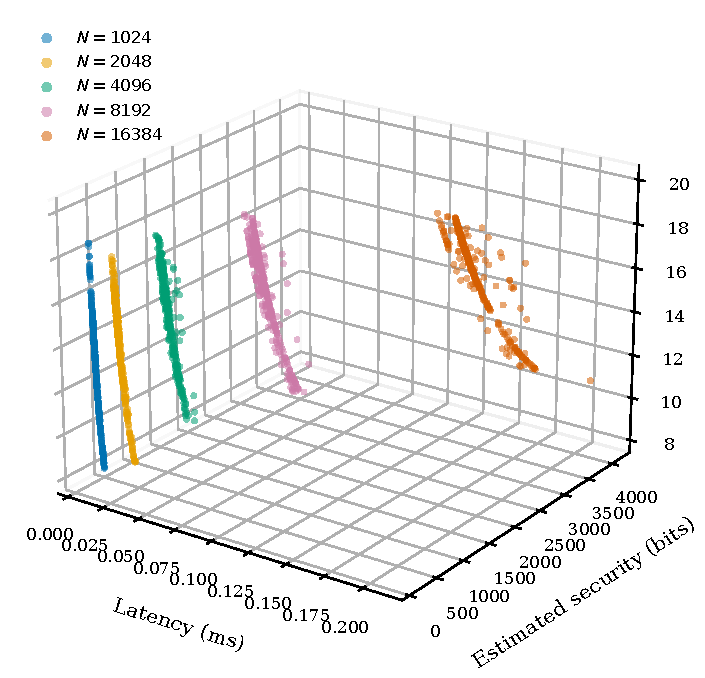
\includegraphics[width=0.95\linewidth,height=\textheight,keepaspectratio,alt={Merged frontier in latency × estimated security × noise-budget space, coloured by N tier (n = 2\{,\}026). A static projection of the interactive scatter in viz/index.html. Per-point discovery generation is not recorded in the frontier artefact and is therefore not encoded.}]{figures/fig1-frontier-3d.pdf}
\caption{Merged frontier in latency × estimated security × noise-budget space, coloured by \(N\) tier (\(n = 2{,}026\)). A static projection of the interactive scatter in \protect\texttt{viz/index.html}. Per-point discovery generation is not recorded in the frontier artefact and is therefore not encoded.}\label{fig:frontier-3d}
\end{figure}

\section{Results}\label{results}

The run completed in 12,007.5 seconds (approximately 3 hours 20 minutes) on the platform described in Section 5, executing 10,000 generations in each of the five polynomial degree tiers sequentially on an idle machine. It produced 2,026 frontier genomes in total. Per-tier wall-clock times are not recorded in the run artefacts and are therefore not reported.

\subsection{Pareto Frontier Characteristics}\label{pareto-frontier-characteristics}

Table 1 summarizes the per-tier results as recorded by each tier's own front, i.e.~\textbf{before} the cross-tier merge and deduplication described in Section 3.6. The per-tier fronts total 2,027 genomes; deduplication removes 1, giving the 2,026 of the merged set discussed in Section 6.3. Because populations are stratified by polynomial degree and each tier's front contains only that degree, the merged partition differs from Table 1 only by that single removal.

\textbf{Table 1: Per-tier Pareto front summary (pre-deduplication, per-tier fronts)}

{\def\LTcaptype{none} % do not increment counter
\begin{longtable}[]{@{}
  >{\raggedright\arraybackslash}p{(\linewidth - 8\tabcolsep) * \real{0.1124}}
  >{\raggedright\arraybackslash}p{(\linewidth - 8\tabcolsep) * \real{0.1573}}
  >{\raggedright\arraybackslash}p{(\linewidth - 8\tabcolsep) * \real{0.2135}}
  >{\raggedright\arraybackslash}p{(\linewidth - 8\tabcolsep) * \real{0.2360}}
  >{\raggedright\arraybackslash}p{(\linewidth - 8\tabcolsep) * \real{0.2809}}@{}}
\toprule\noalign{}
\begin{minipage}[b]{\linewidth}\raggedright
Tier (N)
\end{minipage} & \begin{minipage}[b]{\linewidth}\raggedright
Front size
\end{minipage} & \begin{minipage}[b]{\linewidth}\raggedright
Best latency (ms)
\end{minipage} & \begin{minipage}[b]{\linewidth}\raggedright
Best security (estimator bits)
\end{minipage} & \begin{minipage}[b]{\linewidth}\raggedright
Best noise budget (bits)
\end{minipage} \\
\midrule\noalign{}
\endhead
\bottomrule\noalign{}
\endlastfoot
1024 & 487 & 0.008 & 315.9 & 18.7 \\
2048 & 399 & 0.017 & 631.8 & 18.0 \\
4096 & 374 & 0.035 & 1080.7 & 18.9 \\
8192 & 394 & 0.074 & 2045.7 & 19.8 \\
16384 & 373 & 0.159 & 4091.4 & 19.8 \\
\end{longtable}
}

Front sizes are comparable across tiers (373--487 genomes). Best latency scales with \(O(N \log N)\) (Section 6.4). Maximum estimator-bit values grow roughly linearly in \(N\), which is a property of the heuristic of Section 3.3 rather than an independent finding. Best noise budget is tightly clustered (18.0--19.8 bits) and is not a discriminating objective at this scale.

\textbf{Latency is essentially flat in \(q\) at fixed \(N\).} Taking for each distinct modulus the best latency measured at that modulus, with \textbf{no} post-hoc filter, the full spread across the tier is 3.7\% at \(N = 1024\) (all 70 distinct moduli), 8.0\% at \(N = 2048\) (all 75), 9.4\% at \(N = 4096\) (all 75), 8.0\% at \(N = 8192\) (all 78) and 7.7\% at \(N = 16384\) (all 50). Every frontier genome lies within 1.4× of its tier minimum; the \textasciitilde3.3× efficiency-core mode present in a preliminary unpinned run is absent here.

For comparison, the step between adjacent tiers is a factor of roughly 2.15×. The insensitivity is therefore an order of magnitude larger than the residual variation within a tier: modulus choice at fixed \(N\) costs at most 9.4\%, while a single doubling of \(N\) costs 115\%.

The ordering is not by modulus magnitude either. We therefore withdraw any suggestion that large moduli are faster because of favourable Montgomery constants: the frontier's low-latency and high-security extremes are separated primarily by \(\sigma\) and by modulus magnitude acting through the \emph{analytic} security and noise-budget formulas of Section 3.3, not by measured latency.

\textbf{Benchmark threads prefer performance cores; the frontier is uncontaminated.} A preliminary run without core preference produced a sharply bimodal latency distribution --- a minority cluster at approximately 3.3× the tier minimum, with nothing between 1.4× and 3.3× --- matching the performance-to-efficiency throughput ratio on the 12P+4E platform of Section 5. The per-evaluation median alone does not protect against sticky core placement, because placement can persist for the lifetime of an evaluation. The reported run therefore (1) sizes the Rayon benchmark pool to the performance-core count and requests interactive QoS on every worker, and (2) scores each genome as the minimum of three independent medians so a trial that nonetheless lands on an efficiency core does not determine the fitness. Empirically, the slow cluster is gone: max/min latency within each tier is 1.09×--1.36×, zero genomes sit at ≥2.5× the tier minimum, and the unconditioned modulus-insensitivity figures above coincide with what a 1.5× filter would have produced (that filter retains 100\% of genomes).

Fastest configuration per tier, from the merged frontier (\texttt{results/validation-report.txt}):

\begin{itemize}
\tightlist
\item
  \(N = 1024\): \(q = 5{,}324{,}801\), \(\sigma = 7.692\), \(B_g = 8\) → 0.0078 ms, 167.1 estimator bits, 17.4 bits noise budget
\item
  \(N = 2048\): \(q = 724{,}993\), \(\sigma = 8.025\), \(B_g = 134\) → 0.0166 ms, 393.8 estimator bits, 14.5 bits noise budget
\item
  \(N = 4096\): \(q = 638{,}977\), \(\sigma = 10.000\), \(B_g = 8\) → 0.0353 ms, 812.4 estimator bits, 14.0 bits noise budget
\item
  \(N = 8192\): \(q = 6{,}258{,}689\), \(\sigma = 6.701\), \(B_g = 8\) → 0.0737 ms, 1307.7 estimator bits, 17.8 bits noise budget
\item
  \(N = 16384\): \(q = 65{,}537\), \(\sigma = 5.177\), \(B_g = 18\) → 0.1589 ms, 3806.3 estimator bits, 11.6 bits noise budget
\end{itemize}

Several tiers contain multiple genomes tied at the reported minimum latency; the entries above are those selected by \texttt{results/validation-report.txt}, and a different tie-break would name different moduli at the same latency. This is itself an instance of the insensitivity result: at fixed \(N\), the modulus does not determine latency. All five have \(\sigma \geq 3.2\) by construction of the search box (Section 6.7).

\begin{figure}
\centering
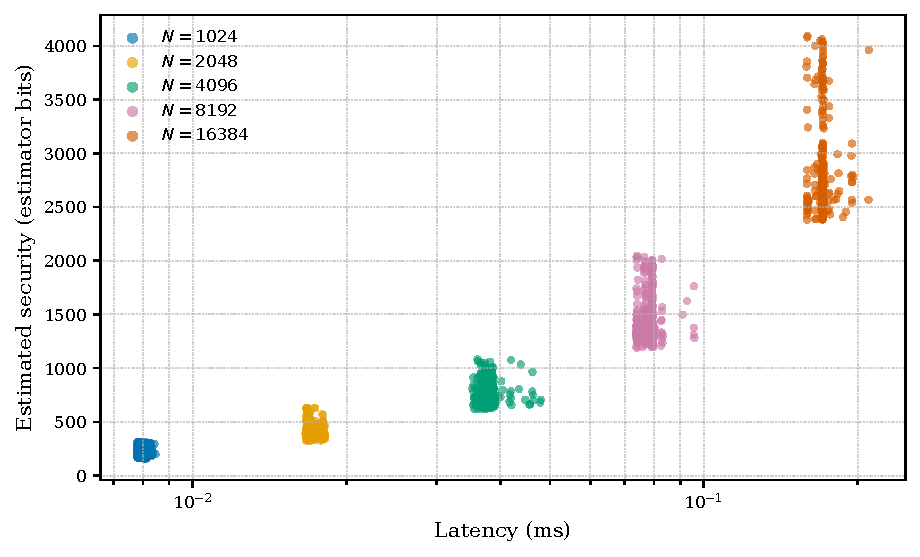
\includegraphics[width=0.95\linewidth,height=\textheight,keepaspectratio,alt={Per-tier fronts projected onto the latency--estimated-security plane (n = 2\{,\}026). The genomes form five clusters, one per polynomial degree tier, with negligible latency spread within each cluster relative to the separation between clusters. Latency axis is logarithmic.}]{figures/fig2-latency-security.pdf}
\caption{Per-tier fronts projected onto the latency--estimated-security plane (\(n = 2{,}026\)). The genomes form five clusters, one per polynomial degree tier, with negligible latency spread within each cluster relative to the separation between clusters. Latency axis is logarithmic.}\label{fig:latency-security}
\end{figure}

\subsection{Convergence Analysis}\label{convergence-analysis}

Best-per-objective values stabilise early --- within 100 generations for four of the five tiers --- while front size continues to fluctuate for thousands of additional generations. Values below are read from \texttt{results/convergence.json}, which records aggregates every 100 generations.

\begin{itemize}
\tightlist
\item
  \textbf{\(N = 1024\)}: best latency 0.007750 ms at Generation 0, ending at 0.007792 ms after 10,000 generations --- a 0.5\% \emph{increase}, i.e.~within measurement noise and not an improvement. Front size grows from 283 to 487 and best estimator output reaches 315.9, so the search expands frontier coverage without improving the latency optimum. The tier's search space is 50 candidate primes crossed with the \(\sigma\) and \(B_g\) ranges; it is not exhaustively or near-exhaustively covered, and we make no such claim.
\end{itemize}

\textbf{Evolutionary search does not improve the latency optimum, in any tier.} This is not specific to \(N = 1024\). Comparing Generation 0 against Generation 9,999:

{\def\LTcaptype{none} % do not increment counter
\begin{longtable}[]{@{}
  >{\raggedright\arraybackslash}p{(\linewidth - 10\tabcolsep) * \real{0.1667}}
  >{\raggedright\arraybackslash}p{(\linewidth - 10\tabcolsep) * \real{0.1667}}
  >{\raggedright\arraybackslash}p{(\linewidth - 10\tabcolsep) * \real{0.1667}}
  >{\raggedright\arraybackslash}p{(\linewidth - 10\tabcolsep) * \real{0.1667}}
  >{\raggedright\arraybackslash}p{(\linewidth - 10\tabcolsep) * \real{0.1667}}
  >{\raggedright\arraybackslash}p{(\linewidth - 10\tabcolsep) * \real{0.1667}}@{}}
\toprule\noalign{}
\begin{minipage}[b]{\linewidth}\raggedright
Tier (N)
\end{minipage} & \begin{minipage}[b]{\linewidth}\raggedright
Gen 0 (ms)
\end{minipage} & \begin{minipage}[b]{\linewidth}\raggedright
Gen 9,999 (ms)
\end{minipage} & \begin{minipage}[b]{\linewidth}\raggedright
Best ever (ms)
\end{minipage} & \begin{minipage}[b]{\linewidth}\raggedright
Change
\end{minipage} & \begin{minipage}[b]{\linewidth}\raggedright
Front size
\end{minipage} \\
\midrule\noalign{}
\endhead
\bottomrule\noalign{}
\endlastfoot
1024 & 0.007750 & 0.007792 & 0.007500 & +0.5\% & 283 → 487 \\
2048 & 0.016666 & 0.016625 & 0.016271 & −0.3\% & 297 → 399 \\
4096 & 0.035292 & 0.035250 & 0.034125 & −0.1\% & 270 → 374 \\
8192 & 0.073688 & 0.073708 & 0.070875 & +0.03\% & 261 → 394 \\
16384 & 0.158625 & 0.158917 & 0.153250 & +0.2\% & 211 → 373 \\
\end{longtable}
}

Ten thousand generations move best latency by between −0.3\% and +0.5\%, which is within the run-to-run variance of the measurement itself. In every tier the best latency ever observed is within a few percent of what the initial random population already contained. What the search demonstrably does is expand frontier coverage: front sizes grow by 34--72\%.

This is the insensitivity result observed from the optimiser's side, and it is the more useful statement of it. If latency is nearly flat in \(q\), \(\sigma\) and \(B_g\) at fixed \(N\), then there is almost nothing in that objective for an evolutionary algorithm to find, and random sampling of the prime pool is sufficient to locate the latency optimum. The honest conclusion is that NSGA-II is doing multi-objective \emph{frontier construction} here, not latency optimisation --- and that a practitioner wanting only the fastest configuration at a given \(N\) can obtain it by sampling the modulus pool, without an evolutionary search at all.
- \textbf{\(N = 2048\)}: best latency 0.016 ms from Generation 100; front size in the 400--420 range.
- \textbf{\(N = 4096\)}: best latency 0.034 ms from Generation 100; front size around 420--440.
- \textbf{\(N = 8192\)}: best latency 0.072 ms from Generation 100; front size around 410--440.
- \textbf{\(N = 16384\)}: best latency reached 0.154--0.155 ms by Generation 700; front size around 380--400.

Early stabilisation of the objective extrema, with front size drifting thereafter, is consistent with the observation in Section 6.1 that within a tier the objectives are nearly analytic functions of \((q, \sigma)\): once the boundary configurations are found, further generations redistribute genomes along an essentially fixed surface. Front size is a weak quality indicator [14] and we do not interpret its drift as improvement.

\begin{figure}
\centering
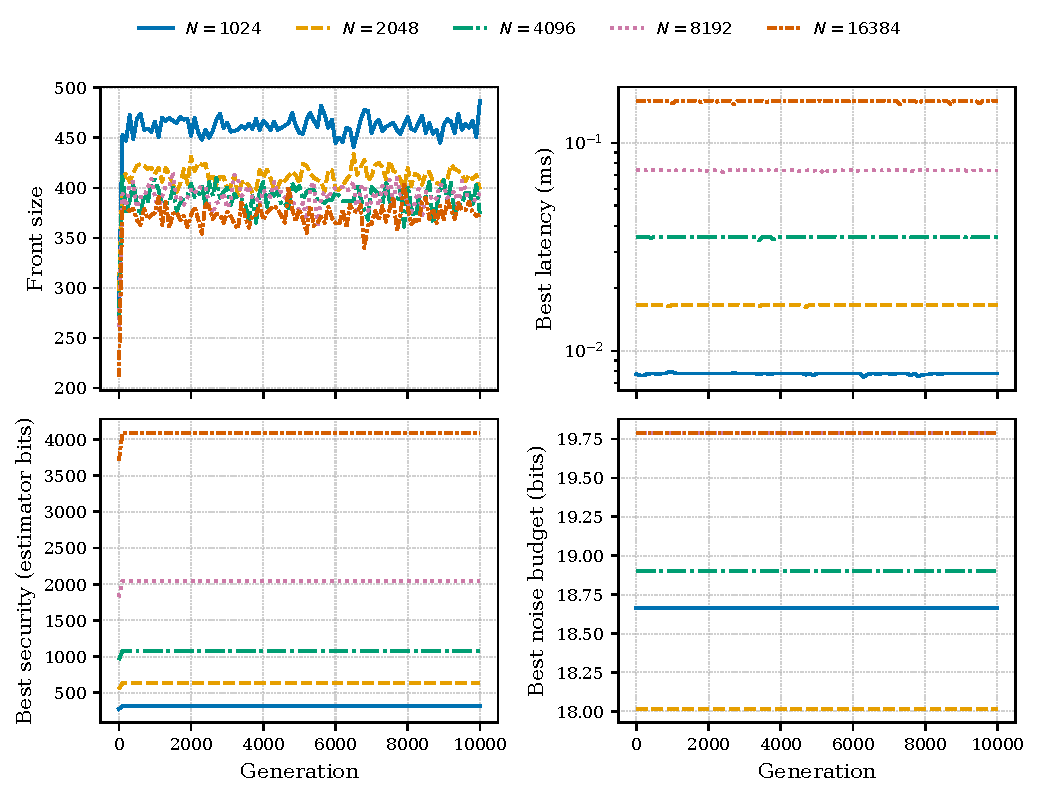
\includegraphics[width=0.95\linewidth,height=\textheight,keepaspectratio,alt={Convergence traces from results/convergence.json: per-100-generation front size and best-per-objective values for each tier. Hypervolume was not computed; the artefact records only the aggregates shown.}]{figures/fig3-convergence.pdf}
\caption{Convergence traces from \protect\texttt{results/convergence.json}: per-100-generation front size and best-per-objective values for each tier. Hypervolume was not computed; the artefact records only the aggregates shown.}\label{fig:convergence}
\end{figure}

\subsection{Comparison to HE Standard 2018}\label{comparison-to-he-standard-2018}

Of the 2,026 merged-frontier genomes, none exceeds the HE Standard 2018 maximum \(\log_2(q)\) for its polynomial degree. The merged set partitions as 486 / 399 / 374 / 394 / 373 genomes for \(N = 1024\) through \(16384\) (post-deduplication; contrast the pre-deduplication per-tier counts in Table 1).

The maximum \(\log_2(q)\) anywhere on the frontier is 23.47, and the minimum is 13.59 --- the whole frontier occupies \(\log_2(q) \in [13.6, 23.5]\), well inside the standard's most restrictive allowance of 27 bits at \(N = 1024\). This is a direct consequence of how the search was posed rather than a discovery about the hardware: the prime pool is enumerated upward from \(q = 2kN + 1\) with \(k = 1\) and capped at 50 entries per tier (Section 4.3), so the largest modulus available at any tier is around \(2^{23.5}\). The frontier could not have contained larger moduli. Combined with the flatness result of Section 6.1, the correct reading is that modulus magnitude in this range does not trade against latency at all, so the search had no latency incentive to move either way within the pool.

The highest estimator-bit configurations per tier, from the per-tier fronts (\texttt{results/summary.txt}):

\begin{itemize}
\tightlist
\item
  \(N = 1024\): \(q = 12{,}289\), latency 0.008 ms → 315.9 estimator bits
\item
  \(N = 2048\): \(q = 12{,}289\), latency 0.017 ms → 631.8 estimator bits
\item
  \(N = 4096\): \(q = 40{,}961\), latency 0.036 ms → 1080.7 estimator bits
\item
  \(N = 8192\): \(q = 65{,}537\), latency 0.074 ms → 2045.7 estimator bits
\item
  \(N = 16384\): \(q = 65{,}537\), latency 0.160 ms → 4091.4 estimator bits
\end{itemize}

These are outputs of the heuristic described in Section 3.3, evaluated far outside its single calibration point. They indicate a large margin in the heuristic's own ordering; they are not calibrated bit-security figures and should not be read as multiples of the 128-bit floor. Section 6.7 restates this limitation.

\textbf{Table 2: Evolved moduli vs.~HE Standard 2018 bounds}

{\def\LTcaptype{none} % do not increment counter
\begin{longtable}[]{@{}
  >{\raggedright\arraybackslash}p{(\linewidth - 6\tabcolsep) * \real{0.0441}}
  >{\raggedright\arraybackslash}p{(\linewidth - 6\tabcolsep) * \real{0.4118}}
  >{\raggedright\arraybackslash}p{(\linewidth - 6\tabcolsep) * \real{0.3529}}
  >{\raggedright\arraybackslash}p{(\linewidth - 6\tabcolsep) * \real{0.1912}}@{}}
\toprule\noalign{}
\begin{minipage}[b]{\linewidth}\raggedright
N
\end{minipage} & \begin{minipage}[b]{\linewidth}\raggedright
HE Standard max \(\log_2(q)\)
\end{minipage} & \begin{minipage}[b]{\linewidth}\raggedright
Evolved max \(\log_2(q)\)
\end{minipage} & \begin{minipage}[b]{\linewidth}\raggedright
Utilisation
\end{minipage} \\
\midrule\noalign{}
\endhead
\bottomrule\noalign{}
\endlastfoot
1024 & 27 & 22.3 & 83\% \\
2048 & 54 & 21.7 & 40\% \\
4096 & 109 & 22.6 & 21\% \\
8192 & 218 & 23.5 & 11\% \\
16384 & 438 & 23.5 & 5\% \\
\end{longtable}
}

Values in the ``Evolved max'' column are taken from \texttt{results/summary.txt}. The compliance statement in this section concerns \(\log_2(q)\); separately, all 2,026 frontier genomes also satisfy \(\sigma \geq 3.2\) by construction of the search box (Section 6.7).

\subsection{Modular Reduction Strategy and Scaling Behaviour}\label{modular-reduction-strategy-and-scaling-behaviour}

To characterise where NTT performance actually comes from on this platform, we measured four reduction strategies within a single library (\texttt{node-fhe-accelerate}) using that library's own benchmark harness, on an idle machine. This is a controlled intra-library comparison: only the reduction strategy varies. The transform measured is the genuine negacyclic NTT over \(\mathbb{Z}_q[X]/(X^N + 1)\) --- a \(\psi\) twist followed by the cyclic core with \(\omega = \psi^2\), where \(\psi\) is a primitive \(2N\)-th root of unity.

The measurement is reported at \textbf{two moduli}. The Metal kernels of Section 6.5 use \(R = 2^{32}\) Montgomery arithmetic and refuse any modulus at or above \(2^{32}\) (Section 6.7), while FHE needs 50--60 bit moduli. Table 3a, at \(q = 2^{60} - 2^{18} + 1\), is therefore the FHE-realistic characterisation; Table 3b, at \(q = 132{,}120{,}577\), exists so that the GPU comparison of Section 6.5 is apples-to-apples. Both tables give cross-session medians over 4 independent sessions with min--max ranges, from 100 timed iterations after 10 warmup iterations per session, and every row passes the correctness gate described at the end of this subsection.

\textbf{Table 3a: CPU negacyclic NTT, \(q = 2^{60} - 2^{18} + 1\) (60-bit), µs, median (min--max)}

{\def\LTcaptype{none} % do not increment counter
\begin{longtable}[]{@{}
  >{\raggedright\arraybackslash}p{(\linewidth - 8\tabcolsep) * \real{0.2000}}
  >{\raggedright\arraybackslash}p{(\linewidth - 8\tabcolsep) * \real{0.2000}}
  >{\raggedright\arraybackslash}p{(\linewidth - 8\tabcolsep) * \real{0.2000}}
  >{\raggedright\arraybackslash}p{(\linewidth - 8\tabcolsep) * \real{0.2000}}
  >{\raggedright\arraybackslash}p{(\linewidth - 8\tabcolsep) * \real{0.2000}}@{}}
\toprule\noalign{}
\begin{minipage}[b]{\linewidth}\raggedright
N
\end{minipage} & \begin{minipage}[b]{\linewidth}\raggedright
Scalar
\end{minipage} & \begin{minipage}[b]{\linewidth}\raggedright
NEON
\end{minipage} & \begin{minipage}[b]{\linewidth}\raggedright
Barrett
\end{minipage} & \begin{minipage}[b]{\linewidth}\raggedright
Montgomery
\end{minipage} \\
\midrule\noalign{}
\endhead
\bottomrule\noalign{}
\endlastfoot
1024 & 34.34 (33.86--35.32) & 34.92 (33.87--35.58) & 14.89 (14.86--14.92) & 7.98 (7.84--8.95) \\
4096 & 220.61 (219.53--224.02) & 216.25 (213.61--217.17) & 70.54 (69.96--71.58) & 37.51 (37.08--38.40) \\
16384 & 1194.39 (1191.28--1199.29) & 1200.86 (1192.80--1205.21) & 416.25 (394.01--423.30) & 174.75 (173.05--177.18) \\
\end{longtable}
}

Montgomery over scalar: 4.30×, 5.88×, 6.84×.

\textbf{Table 3b: CPU negacyclic NTT, \(q = 132{,}120{,}577\) (27-bit), µs, median (min--max)}

{\def\LTcaptype{none} % do not increment counter
\begin{longtable}[]{@{}
  >{\raggedright\arraybackslash}p{(\linewidth - 8\tabcolsep) * \real{0.2000}}
  >{\raggedright\arraybackslash}p{(\linewidth - 8\tabcolsep) * \real{0.2000}}
  >{\raggedright\arraybackslash}p{(\linewidth - 8\tabcolsep) * \real{0.2000}}
  >{\raggedright\arraybackslash}p{(\linewidth - 8\tabcolsep) * \real{0.2000}}
  >{\raggedright\arraybackslash}p{(\linewidth - 8\tabcolsep) * \real{0.2000}}@{}}
\toprule\noalign{}
\begin{minipage}[b]{\linewidth}\raggedright
N
\end{minipage} & \begin{minipage}[b]{\linewidth}\raggedright
Scalar
\end{minipage} & \begin{minipage}[b]{\linewidth}\raggedright
NEON
\end{minipage} & \begin{minipage}[b]{\linewidth}\raggedright
Barrett
\end{minipage} & \begin{minipage}[b]{\linewidth}\raggedright
Montgomery
\end{minipage} \\
\midrule\noalign{}
\endhead
\bottomrule\noalign{}
\endlastfoot
1024 & 21.74 (21.07--22.46) & 22.87 (22.76--23.11) & 14.87 (14.77--15.05) & 7.92 (7.91--8.13) \\
4096 & 100.30 (98.57--100.98) & 104.57 (103.92--107.64) & 71.81 (70.61--76.17) & 37.13 (36.81--37.71) \\
16384 & 459.92 (457.91--460.93) & 484.74 (481.89--491.23) & 438.16 (416.22--463.90) & 174.72 (174.15--175.69) \\
\end{longtable}
}

Montgomery over scalar: 2.75×, 2.70×, 2.63×.

Four findings follow.

\textbf{Montgomery NTT latency is invariant to modulus width.} The Montgomery column is 7.98 µs against 7.92 µs at \(N = 1024\), 37.51 against 37.13 at \(N = 4096\), and 174.75 against 174.72 at \(N = 16384\) --- across a 33-bit difference in modulus width. This is a considerably stronger form of the flatness result of Section 6.1: on the tuned path, cost is flat not merely across the moduli available within a tier but across modulus \emph{width}. For the fast path, then, the choice of \(q\) is free in latency terms over the whole range a practitioner would consider, from toy moduli to production 60-bit primes.

\textbf{The apparent speedup is a property of the baseline, not of the fast path.} Montgomery's advantage over scalar collapses from 4.30×--6.84× at 60 bits to 2.63×--2.75× at 27 bits, and it does so entirely because scalar gets roughly 2.6× cheaper when the 128-bit reduction shortens --- the Montgomery column barely moves. Any ``up to 6.8×'' claim is therefore a 60-bit-modulus claim and must be labelled as one. Note also that the trend reverses direction with \(N\): the advantage rises with \(N\) at 60 bits (4.30× → 5.88× → 6.84×) and is flat-to-falling at 27 bits (2.75× → 2.70× → 2.63×).

\textbf{NEON's sign is modulus-dependent.} At 60 bits, NEON is parity within noise --- 0.98×, 1.02× and 1.00× relative to scalar. At 27 bits it is a consistent regression: 0.950×, 0.959× and 0.949×, with all four sessions on the same side and cross-session ranges of 1.5--3.6\%, so the sign is real rather than an artefact of one session. The mechanism is the one previously reported: NEON has no native 64×64→128 widening multiply, so the widening multiply at the heart of the butterfly cannot be vectorised, and what remains is load/store vectorisation, which is not the bottleneck. What is new is that the effect now has a measured sign rather than merely parity, and that the sign depends on the modulus. The performance win on this platform comes from cheaper reduction, not from vector width.

\textbf{Barrett's NTT advantage nearly vanishes at 27 bits.} Barrett is 2.31×, 3.13× and 2.87× over scalar at 60 bits, against 1.46×, 1.40× and 1.05× at 27 bits. At \(N = 16384\) on the 27-bit modulus it is within noise of scalar (438.16 µs against 459.92 µs) and is the noisiest row in the whole set, with a cross-session range of 416.22--463.90 µs.

\textbf{Standalone modular multiplication.} Measured separately in the same harness, Barrett Unrolled (4×) over scalar, cross-session medians:

{\def\LTcaptype{none} % do not increment counter
\begin{longtable}[]{@{}lll@{}}
\toprule\noalign{}
n & 60-bit & 27-bit \\
\midrule\noalign{}
\endhead
\bottomrule\noalign{}
\endlastfoot
1024 & 3.61× & 2.17× \\
4096 & 4.60× & 2.07× \\
16384 & 5.36× & 2.06× \\
65536 & 4.70× & 1.35× \\
\end{longtable}
}

Barrett is \textbf{no longer the fastest modmul at the largest size on the 27-bit modulus}: at \(n = 65536\), Barrett Unrolled is 160.93 µs against Montgomery at 144.13 µs and the reducer the harness labels ``Neural Engine'' at 119.43 µs --- a label we report without endorsing, for the reasons given in Section 2.4. The claim that Barrett is fastest for isolated modmul survives for \(n \leq 16384\) at both moduli, and at all sizes measured on the 60-bit modulus, but it inverts at \(n = 65536\) on the 27-bit modulus. The reason the NTT and standalone-modmul orderings differ at all is unchanged: the NTT keeps values in the Montgomery domain across all \(\log_2 N\) stages, so the two domain conversions are amortised over the whole transform, whereas isolated modmul must convert on every operation and therefore pays conversion cost per multiply.

\textbf{Provenance.} Roots of unity were found by search and their order verified (\(g = 10\) for the 60-bit prime, \(g = 5\) for \(q = 132{,}120{,}577\)), the RNG seed 1592598350 is recorded, and each session ran 100 timed iterations after 10 warmup iterations. Every row above is gated on the negacyclic convolution identity described in Section 6.6 --- pointwise product in the transform domain against an independently computed schoolbook negacyclic convolution, with index \(N - 1\) populated in both operands so that the \(X^N = -1\) sign flip is exercised --- and the harness exits non-zero on any failure.

These measurements use the library's own harness. Our Rust implementation's latencies (Section 6.1) are consequently \textbf{not} directly comparable to Table 3a or Table 3b: the moduli differ, we time a forward-only transform rather than a full transform, and the harnesses differ --- even though both sides now measure negacyclic NTTs on an idle machine. We make no claim of an advantage over any third-party backend.

\textbf{Cross-tier scaling.} The best latencies of Section 6.1 track \(O(N \log N)\) closely. Note that the theoretical ratio \((N_2 \log_2 N_2)/(N_1 \log_2 N_1)\) is not constant across transitions; it declines from 2.200 to 2.154.

{\def\LTcaptype{none} % do not increment counter
\begin{longtable}[]{@{}llll@{}}
\toprule\noalign{}
Tier transition & Observed ratio & Theoretical ratio & Deviation \\
\midrule\noalign{}
\endhead
\bottomrule\noalign{}
\endlastfoot
1024 → 2048 & 2.134 & 2.200 & −3.0\% \\
2048 → 4096 & 2.120 & 2.182 & −2.8\% \\
4096 → 8192 & 2.091 & 2.167 & −3.5\% \\
8192 → 16384 & 2.156 & 2.154 & +0.1\% \\
\end{longtable}
}

The independent Montgomery measurements corroborate this: Table 3b gives 174.72 µs at \(N = 16384\) against 7.92 µs at \(N = 1024\), a ratio of 22.06× against a theoretical 22.4× for \(1024 \rightarrow 16384\), a deviation of −1.5\%, and Table 3a gives the same behaviour at 60 bits. Deviations in both datasets are within measurement variance, and no cache-hierarchy or memory-bandwidth cliff was observed up to \(N = 16384\). We offer no micro-architectural explanation for the small negative bias in the four-transition table; none is supported by the data collected.

\subsection{Validated Metal GPU Batch NTT}\label{validated-metal-gpu-batch-ntt}

Earlier drafts of this paper excluded the Metal compute-shader NTT from all results because its output had never been checked against a trusted reference. Several correctness defects were subsequently identified and fixed, the kernel now computes the negacyclic transform, and it is validated against a gate that a wrong transform cannot pass. We report it here, with the validation methodology stated first because it is what makes the numbers admissible.

\textbf{Corrections to the kernel.} \texttt{NTTParams} now carries a genuine Montgomery constant \(q_{\text{inv\_neg}} = -q^{-1} \bmod 2^{32}\), computed by five Newton iterations and verified to satisfy \(q \cdot q_{\text{inv\_neg}} \equiv \text{0xFFFFFFFF}\); the previous version misused \(n^{-1}\) in that role, which cannot produce a correct reduction. Twiddle indexing was corrected to a flat stage-major table of \(N - 1\) entries in which stage \(s\) owns \(m = 2^s\) entries at base \(2^s - 1\), addressed by position \emph{within} the butterfly group (\texttt{stage\_base\ +\ offset}) rather than by group index; the previous expression reached index 261,632 into a 1,024-element buffer. The \(R = 2^{64}\) helpers, which contained a \texttt{\textgreater{}\textgreater{}\ 64} shift, were deleted and replaced by \(R = 2^{32}\) Montgomery arithmetic (\texttt{mont\_mul\_32} / \texttt{mont\_redc\_32}), which is exact in 64 bits because every modulus in this study is odd and below \(2^{32}\). The \emph{contents} of the twiddle table were also wrong, and that defect is the subject of Section 6.6: the table held powers of the primitive \(2N\)-th root \(\psi\) while the butterfly schedule consumes powers of the \(N\)-th root \(\omega = \psi^2\), so every exponent was halved. Both the CPU reference and the GPU port now build the table from \(\omega\), with the \(\psi\) twist applied explicitly, giving the genuine negacyclic transform over \(\mathbb{Z}_q[X]/(X^N + 1)\). Separately, the transform encodes conversion to Montgomery form, bit-reversal permutation, all \(\log_2 N\) butterfly stages, optional \(N^{-1}\) scaling, and conversion out of Montgomery form into a \textbf{single command buffer} with one commit and one wait, in place of \(\log_2(N) + 1\) separate command buffers each carrying its own \texttt{waitUntilCompleted}. The transform refuses outright --- returning false and leaving the caller's buffer untouched --- when \(q\) is even, when \(q \geq 2^{32}\), or when \(N\) has no inverse modulo \(q\).

\textbf{Validation.} Every configuration is gated twice. First, the negacyclic convolution identity of Section 6.6: the pointwise product of two transformed operands must match an independently computed schoolbook negacyclic convolution, with index \(N - 1\) populated in both operands so that the \(X^N = -1\) sign flip is exercised. Second, coefficient-exact agreement with the CPU reference for every polynomial in the batch. Across the 20 independent runs reported below, all 280 configuration-results pass both checks; the process exits non-zero and names the failing configuration otherwise. The unit suite described in Section 4.4 covers the small-degree, small-batch and refusal cases that the benchmark configurations do not reach.

\textbf{Modulus.} All configurations use \(q = 132{,}120{,}577 = 63 \cdot 2^{21} + 1\), for which \(2N \mid q - 1\) for every \(N\) up to \(2^{20}\). Every configuration reported here is therefore negacyclic-valid --- the same \(q \equiv 1 \pmod{2N}\) condition satisfied by every genome on the evolutionary frontier (Section 6.7). This is checked at runtime per configuration and reported in the harness output.

\textbf{Table 4: Validated Metal GPU batch negacyclic NTT against the in-process CPU reference oracle. Medians of 20 runs; the GPU range column gives min--max over those runs; relative IQR is IQR/median. Quantiles are linear-interpolated.}

{\def\LTcaptype{none} % do not increment counter
\begin{longtable}[]{@{}lllllll@{}}
\toprule\noalign{}
N & Batch & CPU ref (µs) & GPU (µs) & GPU range & rel IQR & Speedup \\
\midrule\noalign{}
\endhead
\bottomrule\noalign{}
\endlastfoot
1024 & 16 & 28.91 & 16.18 & 15.65--16.54 & 1.7\% & 1.8× \\
1024 & 256 & 28.81 & 2.05 & 2.00--2.08 & 1.5\% & 14.1× \\
1024 & 512 & 29.05 & 1.59 & 1.56--1.63 & 0.9\% & 18.3× \\
1024 & 1024 & 29.32 & 1.34 & 1.32--1.37 & 1.5\% & 21.9× \\
2048 & 128 & 63.16 & 4.54 & 4.45--4.73 & 1.4\% & 13.9× \\
2048 & 256 & 63.73 & 3.50 & 3.43--3.64 & 2.1\% & 18.2× \\
2048 & 512 & 63.91 & 2.98 & 2.87--3.18 & 3.1\% & 21.5× \\
4096 & 64 & 136.56 & 9.96 & 9.67--10.19 & 1.2\% & 13.7× \\
4096 & 128 & 136.92 & 7.51 & 7.28--7.91 & 3.5\% & 18.2× \\
4096 & 256 & 138.53 & 6.28 & 6.10--7.60 & 4.9\% & 22.1× \\
8192 & 32 & 293.42 & 22.46 & 21.79--23.45 & 3.9\% & 13.1× \\
8192 & 64 & 295.65 & 16.56 & 16.19--17.41 & 3.7\% & 17.9× \\
16384 & 16 & 636.57 & 53.34 & 51.98--57.21 & 4.1\% & 11.9× \\
16384 & 32 & 636.77 & 38.02 & 36.55--47.91 & 3.3\% & 16.8× \\
\end{longtable}
}

\textbf{The speedup in Table 4 must not be taken as the headline figure.} The ``CPU ref'' column is \texttt{NTTProcessor::forward\_ntt}, the in-process path used as the correctness oracle. It is not the fastest CPU NTT available on this machine. At \(N = 1024\) the oracle is 29.32 µs against 7.92 µs for the tuned Montgomery path of Table 3b --- a factor of 3.7×, wider than the gap reported before the corrections. Quoting the 12--22× oracle-relative band would therefore overstate the GPU advantage by attributing to the GPU a gap that is partly an artefact of the baseline. We report both ratios and lead with the conservative one.

\textbf{Table 5: Best GPU result against the fastest measured CPU NTT, both at \(q = 132{,}120{,}577\), both negacyclic. CPU values are the Montgomery column of Table 3b; GPU values are medians of 20 runs.}

{\def\LTcaptype{none} % do not increment counter
\begin{longtable}[]{@{}lllll@{}}
\toprule\noalign{}
N & Fastest CPU (Table 3b) & Best GPU & Batch & Speedup \\
\midrule\noalign{}
\endhead
\bottomrule\noalign{}
\endlastfoot
1024 & 7.92 & 1.34 & 1024 & 5.9× \\
4096 & 37.13 & 6.28 & 256 & 5.9× \\
16384 & 174.72 & 38.02 & 32 & 4.6× \\
\end{longtable}
}

\textbf{4.6×--5.9× over the fastest measured CPU path is the defensible figure.} It is also, for the first time, a like-for-like comparison: both sides run at the same modulus, both compute the same negacyclic transform, and each side is independently gated on the convolution identity. The previous version of this table compared different transforms at different moduli and should be discarded. The oracle-relative band is 12--22×, and because the oracle is now 3.7× slower than the tuned path, the gap between the two baselines is wider than before --- which is precisely why the conservative figure is the one to lead with.

Four further observations follow from the data.

\textbf{1. Batch amortisation, and the knee was never reached.} Per-NTT cost is monotone decreasing in batch size at every degree: at \(N = 2048\) it runs 4.54 → 3.50 → 2.98 µs from batch 128 to batch 512, and at \(N = 1024\) from 16.18 µs at batch 16 down to 1.34 µs at batch 1024. The largest batch tested wins at every degree, so no interior optimum was found and the device remains dispatch-bound at the top of the sweep; the batch sizes at which the GPU saturates are above those measured. The single-command-buffer design bounds the fixed cost at one synchronisation per transform regardless of \(N\), rather than one per stage. Note that an earlier draft claimed per-NTT cost stops improving by batch 256 at \(N = 2048\). That claim does not survive correction --- it was an artefact of the degenerate transform and of noise in a five-run sample --- and it is withdrawn.

\textbf{2. Speedup against the best CPU path falls only at the largest degree.} 5.9× at \(N = 1024\), 5.9× at \(N = 4096\), 4.6× at \(N = 16384\). The first two are identical to two significant figures. Larger \(N\) means fewer polynomials fit within the batch sizes tested and a larger per-transform working set; we assert no specific micro-architectural cause, having measured none.

\textbf{3. The negacyclic twist costs 1.4\%--17.2\%, measured by in-process A/B.} Same process, same data, interleaved repetitions of a cyclic arm against a negacyclic arm: +1.4\% at \(N = 1024\), +3.0\% at \(N = 2048\), +2.1\% at \(N = 4096\), +8.6\% at \(N = 8192\) and +17.2\% at \(N = 16384\). The twist adds no dispatch and no synchronisation --- it is fused into the Montgomery domain crossing that already runs --- so what is being paid is bandwidth: at \(N = 16384\) the twist table is 128 KB and is re-read per threadgroup, which is why the cost concentrates at the top two degrees. The methodological point is worth stating explicitly, because it is easy to get backwards: this had to be measured \emph{within a single process}. Comparing the corrected run against the pre-fix archived run shows the \textbf{opposite} sign --- medians fell by 10--15\% --- purely because the machine was 10--25\% faster on the later day. Cross-run differences cannot attribute cost to a code change, however large the sample on either side.

\textbf{4. Repeatability is now good, and the remaining variance is single-outlier rather than broad.} Relative IQR is at or below 4.9\% at all fourteen configurations, against up to 34\% in the pre-fix data. The widest total spread is \((N, \text{batch}) = (16384, 32)\) at 29.9\%, and it is entirely attributable to one 47.91 µs sample against a 3.3\% IQR. The general lesson is that relative spread and median stability measure different things: ranking configurations by total spread alone misidentifies which numbers are trustworthy, since a single scheduling outlier inflates the spread of an otherwise tight distribution. We report both, and we report the full range so that outliers remain visible rather than being absorbed into a summary statistic.

\subsection{Round-Trip Verification Is Insufficient}\label{round-trip-verification-is-insufficient}

Every measurement in the previous versions of Sections 6.4 and 6.5 timed a transform that was not an NTT, and every one of them passed round-trip verification. The reason is structural rather than accidental, and it is worth stating as a theorem because it invalidates a verification practice that is close to universal in implementation work.

\textbf{For any twiddle table with nonzero entries, a Cooley--Tukey forward pass composed with a Gentleman--Sande inverse pass whose table is the elementwise inverse of the forward table --- entry by entry, \(t \mapsto t^{-1}\) --- recovers the input exactly.} The forward butterfly is \(\begin{pmatrix} 1 & t \\ 1 & -t \end{pmatrix}\) and its inverse-pass counterpart is \(\begin{pmatrix} 1 & 1 \\ t^{-1} & -t^{-1} \end{pmatrix}\); their product is \(2 I\) for \textbf{every} \(t \neq 0\), with no dependence on \(t\) whatsoever. Over \(\log_2 N\) stages the composition is \(N \cdot I\), and the \(N^{-1}\) scaling applied by the inverse transform cancels it exactly. A forward/inverse pair built from an all-ones twiddle table round-trips perfectly. Round-tripping therefore establishes that the forward and inverse passes are mutual inverses; it establishes nothing about \emph{which} transform they compute, and in particular it cannot detect a wrong twiddle table.

The elementwise-inverse precondition is not a loophole that narrows the result; it is the normal case. If the two tables were built from unrelated roots the composition would not be diagonal and the round-trip would fail --- but no implementation examined here did that, and few would: every one of them derived its inverse table from its forward table by inverting each entry, which is the obvious construction and is close to universal. The precondition is thus satisfied by default rather than being a condition one has to arrange, and that is precisely why all four defective transforms below round-tripped.

Porting the fix into the Rust sandbox surfaced a second failure mode in the same family: \textbf{omitting the \(\psi\) twist altogether}. What remains is a perfectly valid cyclic NTT --- it round-trips exactly, and its twiddles are genuine powers of a root of the correct order \(N\), so an order check at the point of root selection passes as well --- but it convolves modulo \(X^N - 1\) instead of \(X^N + 1\). This is arguably the more dangerous of the two, because nothing about the transform is malformed: it is a correct transform of the wrong ring, and only the convolution identity distinguishes it.

This is not hypothetical. Four instances were found in this codebase, and the split between them matters: two sat in code paths that produced published numbers --- the hardcoded \texttt{find\_primitive\_root} returning 3, and the twiddle table built from \(\psi\) where the butterfly schedule consumes \(\omega\) --- while the other two were latent in code that was never linked into a measurement, namely the matrix-form NTT with \(w = 1\) and the inverse transform scaling by \texttt{inv\_n\ =\ 1}. All four passed round-trip verification, and all four had survived review:

\begin{itemize}
\tightlist
\item
  A \texttt{find\_primitive\_root} in the CPU benchmark harness that returned the literal 3 for \(q = 132{,}120{,}577\), a modulus for which 3 is not a generator --- its multiplicative order is \((q-1)/4\). The derived twiddle \(w = 3^{(q-1)/N}\) consequently had order 256 at \(N = 1024\), 1024 at \(N = 4096\) and 4096 at \(N = 16384\), never \(N\).
\item
  A twiddle table in \texttt{NTTProcessor::precompute\_twiddles} filled with powers of the primitive \(2N\)-th root \(\psi\), while the butterfly schedule indexes \(j \cdot (N/\text{group\_size})\), an exponent of the \(N\)-th root \(\omega = \psi^2\). Every exponent was halved, and the resulting transform was neither cyclic nor negacyclic. This one propagated: the Metal path was a faithful port of it, and the GPU correctness gate compared GPU output against that same defective reference, so the gate certified agreement with a defect.
\item
  A matrix-form NTT with \(w = 1\) for every twiddle --- a table of order 1.
\item
  An inverse transform scaling by \texttt{inv\_n\ =\ 1} rather than by \(N^{-1}\).
\end{itemize}

Alongside these we found what is best described as correctness theatre: a \texttt{correctness\_verified} field populated from a hardcoded literal on every row, a verification helper whose body was \texttt{return\ true;} and which was never called from anywhere, and a winner-selection routine that filtered candidates on that literal. None of this is exotic; all of it reads as plausible at review time.

\textbf{The evolutionary sandbox was audited against the same defect and is clean.} We checked the Rust benchmark sandbox of Section 3.4 for every member of this defect class and found none. What protects it is not its round-trip check, which by the argument above protects nothing, but an algebraic verification of the root's \emph{order}, performed at the point where the root is selected: \texttt{find\_primitive\_root} in \texttt{native/src/ntt.rs} scans candidate generators \(g\) upward from 2, forms \(\text{root} = g^{(q-1)/N} \bmod q\), and accepts only when \(\text{root}^{N/2} \neq 1 \pmod q\). Because \(N\) is always a power of two, any order properly dividing \(N\) must also divide \(N/2\), so that single test is sufficient: it proves the order is exactly \(N\). \texttt{forward\_ntt} then derives \(w_{\text{step}} = \omega^{N/\text{len}}\) per stage, and the accelerated path in \texttt{ntt\_accel.rs} builds the same table in Montgomery form, so the sandbox computes a genuine cyclic length-\(N\) NTT and does not share the wrong-order defect. The lesson is that verifying the root's order where the root is chosen costs one modular exponentiation and catches the entire defect class at its source, whereas verifying the transform's output afterwards requires the convolution identity. The sandbox is nonetheless not convolution-gated --- the round-trip remains its only runtime check --- and adding that gate is the remaining verification gap on the CPU side.

\textbf{The gate that works is the convolution identity.} Pointwise multiplication in the transform domain must equal negacyclic convolution in the coefficient domain: \(\text{NTT}^{-1}(\text{NTT}(a) \odot \text{NTT}(b)) = a \ast_{-} b\), with the right-hand side computed independently by schoolbook convolution under \(X^N = -1\). This pins the transform rather than merely proving the two passes are mutually consistent, because the identity holds only when the twiddles are genuine powers of a primitive root of the right order. Two implementation details make it cheap and make it bite: sparse operands keep the reference computation \(O(N)\) rather than \(O(N^2)\), and populating index \(N - 1\) in both operands forces at least one product to wrap, which exercises the \(X^N = -1\) sign flip that distinguishes the negacyclic transform from the cyclic one. Both the CPU and GPU harnesses now apply this gate to every configuration, exit non-zero on failure, and name the failing configuration rather than silently dropping it.

The generalisable claim is narrow but firm: \textbf{an NTT implementation validated only by round-trip is unvalidated}, and the same argument applies unchanged to the FFT, where the butterfly algebra is identical. That round-trip is insufficient is known in principle, and we claim no novelty for the algebra. What this work adds is evidence that it is easy to get wrong in practice --- four independent instances survived review in a single codebase --- and that the failure mode is silent: every defective implementation above produced plausible latencies, scaled as \(O(N \log N)\), and passed the check it was given.

\subsection{Threats to Validity}\label{threats-to-validity}

Several defects and confounds in this study affect how its numbers should be read. We state them in full.

\textbf{1. Objective degeneracy: \(B_g\) affects no objective.} The gadget decomposition base is part of the genome but enters none of the three objectives. \texttt{security-estimator.ts} computes security from \((N, q, \sigma)\) only; the noise-budget formula uses \((q, \sigma)\) only; and the Rust \texttt{benchmark\_genome} reads only the \texttt{n} and \texttt{q} fields of the packed genome. Because \(B_g\) is nonetheless part of the deduplication key, two genomes that are identical in objective space can both persist as frontier points. Measured effect on the merged frontier:

{\def\LTcaptype{none} % do not increment counter
\begin{longtable}[]{@{}
  >{\raggedright\arraybackslash}p{(\linewidth - 8\tabcolsep) * \real{0.2000}}
  >{\raggedright\arraybackslash}p{(\linewidth - 8\tabcolsep) * \real{0.2000}}
  >{\raggedright\arraybackslash}p{(\linewidth - 8\tabcolsep) * \real{0.2000}}
  >{\raggedright\arraybackslash}p{(\linewidth - 8\tabcolsep) * \real{0.2000}}
  >{\raggedright\arraybackslash}p{(\linewidth - 8\tabcolsep) * \real{0.2000}}@{}}
\toprule\noalign{}
\begin{minipage}[b]{\linewidth}\raggedright
Tier
\end{minipage} & \begin{minipage}[b]{\linewidth}\raggedright
Genomes
\end{minipage} & \begin{minipage}[b]{\linewidth}\raggedright
Distinct objective vectors
\end{minipage} & \begin{minipage}[b]{\linewidth}\raggedright
Distinct \((N, q, \sigma)\)
\end{minipage} & \begin{minipage}[b]{\linewidth}\raggedright
Distinct \(q\)
\end{minipage} \\
\midrule\noalign{}
\endhead
\bottomrule\noalign{}
\endlastfoot
1024 & 486 & 465 & 484 & 70 \\
2048 & 399 & 391 & 399 & 75 \\
4096 & 374 & 374 & 374 & 75 \\
8192 & 394 & 393 & 394 & 78 \\
16384 & 373 & 373 & 373 & 50 \\
\textbf{All} & \textbf{2,026} & \textbf{1,996} & \textbf{2,024} & \textbf{150} \\
\end{longtable}
}

Objective vectors are compared after rounding latency to 4 decimals, security to 1 decimal and noise budget to 1 decimal. The inflation is real but small: 2,026 genomes collapse to 1,996 distinct objective vectors (1.5\%), and only 2 genome groups on the whole frontier differ solely in \(B_g\) (2,024 distinct \((N, q, \sigma)\) triples). The remaining collisions are between different \((N, q, \sigma)\) triples that round to the same objective triple. Reported frontier sizes throughout this paper are genome counts, not counts of distinct trade-off points. Note also the modulus counts: 2,026 genomes occupy only 150 distinct moduli, and at \(N = 16384\) all 50 pool primes appear.

\textbf{2. \(\sigma\) is driven to the box bounds.} Under the estimator of Section 3.3, security is strictly increasing in \(\sigma\) and noise budget strictly decreasing in \(\sigma\). There is therefore no interior optimum: \(\sigma\) saturates at the search bounds \([3.2, 10.0]\), and every tier's frontier contains genomes at exactly \(\sigma = 3.200\) and exactly \(\sigma = 10.000\).

This is a limitation of the estimator's functional form rather than a finding about parameters: a monotone objective in a box constraint always optimises at the boundary, so the search recovers the bounds rather than discovering anything about \(\sigma\). It is not a compliance problem --- the lower bound is the HE Standard minimum of Section 2.1, so all 2,026 frontier genomes satisfy \(\sigma \geq 3.2\) by construction, and the analysis of Section 6.3 confirms zero violations in every tier. A study wishing to make a substantive claim about \(\sigma\) would need an estimator with an interior optimum, or a different treatment of \(\sigma\) altogether.

\textbf{3. The negacyclic requirement, and the cost of satisfying it.} FHE operates in \(\mathbb{Z}_q[X]/(X^N + 1)\) and requires a primitive \(2N\)-th root of unity, i.e.~\(q \equiv 1 \pmod{2N}\) --- strictly stronger than the \(q \equiv 1 \pmod{N}\) that suffices for a cyclic transform over \(X^N - 1\). The prime pool of Section 4.3 enumerates \(q = 2kN + 1\), so every modulus it can produce satisfies the negacyclic condition, and the search space contains no cyclic-only moduli. All 2,026 frontier genomes satisfy \(q \equiv 1 \pmod{2N}\), verified per tier (Section 6.3): 486 / 399 / 374 / 394 / 373, with zero exceptions.

The distinction still bears on the reported timings. A negacyclic transform requires an elementwise \(\psi\) twist of \(N\) modular multiplications in addition to the butterfly network, which a cyclic transform of the same length does not. That pass is measured at +1.4\% to +17.2\% depending on degree (Section 6.5, observation 3), and it is included in the latencies reported throughout this paper. Cost models derived from cyclic-only measurements would understate negacyclic cost by that margin.

\textbf{4. Security estimator fidelity.} The heuristic of Section 3.3 is not a lattice attack cost model, contains no BKZ block size or core-SVP term, and is extrapolated far beyond its single calibration anchor. All security figures in this paper are ordinal estimator outputs. They are sufficient for ranking within the search and insufficient for any bit-security claim. This is the most consequential limitation in the study.

\textbf{5. The security sieve exerted no selective pressure.} \texttt{results/convergence.json} records \texttt{secureCount} and \texttt{populationSize} at every logged generation for every tier: across all 505 logged records, \texttt{secureCount} equals 500 of 500 in every case. After seeding, no genome was ever rejected by the 128-bit floor in a logged generation. The sieve functioned as a seeding constraint, not as an active filter, and the 128-bit floor exerted no selective pressure during the run. This follows from the search box: the heuristic is minimised at the largest available modulus and smallest \(\sigma\), giving \(3.166 \times 1024 / \log_2(2^{22.34}/1.0) \approx 145\) estimator bits as the least attainable value at \(N = 1024\), and larger values at every larger \(N\). The constraint is vacuous over the entire box, so no claim should be made that the sieve filtered candidates during evolution.

\textbf{6. Measurement environment.} All evolutionary-frontier timings reported in this paper, and the reduction-strategy and GPU measurements of Sections 6.4--6.5, were collected on an idle machine. Residual within-tier spread on the frontier (max/min up to 1.36× at \(N = 4096\)) is therefore not attributed to competing load; the four-decimal storage of latencies should still not be read as four-decimal accuracy.

\textbf{7. GPU measurement methodology.} The Section 6.5 figures are medians of 20 independent runs of the benchmark binary, reported with the full min--max range and the relative interquartile range. They are medians rather than means, and at \(n = 20\) we quote ranges and IQRs rather than parametric confidence intervals. Repeatability is now good --- relative IQR is at or below 4.9\% at all fourteen configurations --- but the widest total spread, 29.9\% at \((16384, 32)\), shows that single scheduling outliers still occur and that spread and median stability must be read separately. Two distinct CPU baselines remain in play: the in-process correctness oracle and the Table 3b Montgomery path, the latter 3.7× faster than the former at \(N = 1024\). The conservative 4.6×--5.9× is therefore the defensible figure and the 12--22× band is oracle-relative only; quoting the latter without that qualifier attributes a baseline artefact to the device. Set against this, the correctness gates of Section 4.4 and Section 6.6 are what make these numbers admissible at all, and we record that the convolution gate was added only \emph{after} the kernel --- and the reference it was checked against --- were found to be defective. Nothing in the original harness would have detected either defect, and the original gate actively concealed one of them by comparing the GPU against the same defective reference (Section 6.6). The gate exists because the failure occurred, not because it was anticipated.

\textbf{8. The GPU cannot represent an FHE-realistic modulus.} The Metal kernels use \(R = 2^{32}\) Montgomery arithmetic and refuse any modulus at or above \(2^{32}\); the largest value they accept is \(2^{32} - 1\), and the largest NTT-friendly prime below that bound for \(N = 16384\) is 4,294,475,777. FHE uses 50--60 bit moduli. Every GPU figure in this paper is therefore measured at a 27-bit modulus and does not transfer to production parameters without either RNS decomposition into sub-\(2^{32}\) limbs or 64-bit Montgomery arithmetic with emulated 128-bit products. This is a genuine limitation of the implementation rather than of the methodology, and we state it as such: the CPU path is characterised at 60 bits in Table 3a precisely because the GPU path cannot be.

\textbf{9. Correctness gates are asymmetric in strength across the paper.} Both NTT harnesses, CPU and GPU, are now gated on the negacyclic convolution identity of Section 6.6, which is the strongest gate used anywhere in this work. The standalone modular-multiplication verifier is weaker: it samples only the first 1000 elements. Weaker still, some suites in the benchmark binary retain hardcoded correctness flags of the kind described in Section 6.6. Results in this paper should be weighted accordingly --- the Table 3a, Table 3b and Table 4 NTT figures rest on the strong gate, the standalone modmul figures of Section 6.4 on the sampling verifier.

\textbf{10. Thread placement is mitigated, not assumed away.} A preliminary evolutionary run without core preference produced the classic efficiency-core bimodality (\textasciitilde3.3× slow cluster). The reported run applies the remedies of Section 6.1 --- a performance-core-sized Rayon pool with interactive QoS, plus min-of-k medians --- and the artefact is absent from the frontier (zero genomes at ≥2.5× the tier minimum; unconditioned modulus spreads of 3.7--9.4\%). The remaining threat is that QoS is best-effort on macOS: we verify absence of the mode empirically rather than claiming hard affinity.

\section{Discussion}\label{discussion}

\subsection{Implications for FHE Deployment}\label{implications-for-fhe-deployment}

The practical guidance that follows from these measurements is narrower than we initially expected, and clearer for it.

Within a polynomial degree tier, latency does not discriminate between NTT-friendly moduli on this platform (Section 6.1), and on the tuned Montgomery path it does not discriminate on modulus \emph{width} either: 7.98 µs at 60 bits against 7.92 µs at 27 bits for \(N = 1024\), and 174.75 against 174.72 µs for \(N = 16384\) (Section 6.4). Modulus selection can therefore be driven entirely by security and noise-budget requirements, with no latency penalty to trade against, and the guidance extends to the 50--60 bit moduli production FHE actually uses rather than only to the narrow range the frontier explored. For a fixed \(N\), choose \(q\) for the noise budget the circuit needs and the security margin the deployment requires, and expect the NTT cost to be what the tier dictates.

Between tiers, latency is the dominant consideration and it is predictable. Cross-tier scaling reproduced \(O(N \log N)\) to within 3.5\% (Section 6.4), so a practitioner can estimate the cost of moving to a larger \(N\) without measuring. Hardware-aware optimisation is worth the effort at the granularity of \(N\), and at the granularity of the reduction strategy, rather than within a tier. How much the reduction strategy is worth depends on the modulus: Montgomery is 4.30×--6.84× over scalar at 60 bits but only 2.63×--2.75× at 27 bits, and the difference is almost entirely in the scalar baseline, which gets cheaper as the reduction shortens.

Where the reduction strategy is under the practitioner's control --- for example when selecting or configuring a backend --- Tables 3a and 3b give a concrete ordering for this platform: prefer Montgomery for transforms, and do not expect NEON vectorisation alone to help. NEON is parity within noise at 60 bits (0.98×--1.02×) and a consistent regression at 27 bits (0.949×--0.959×), so the qualifier matters: it is not merely neutral. Note also that the Montgomery-first ordering inverts for isolated modular multiplication, so the choice depends on whether values stay in the Montgomery domain across stages --- and that this inversion is itself modulus-dependent, since Barrett loses its lead at \(n = 65536\) on the 27-bit modulus.

For workloads dominated by bootstrapping [12] or by multi-party key structures [13], NTT latency alone is an incomplete cost model; Section 7.2 addresses this.

\subsection{Limitations}\label{limitations}

Beyond the specific validity threats enumerated in Section 6.7, several limitations bound the generalisability of this work.

\textbf{NTT as performance proxy.} NTT latency is a necessary but not sufficient proxy for full FHE operation performance. Real FHE workloads involve key switching (additional NTTs with different parameters), automorphisms, bootstrapping procedures [12], and memory management overhead. A configuration optimal for isolated NTT may not be optimal for a complete FHE pipeline. NTT is a large fraction of the cost in current lattice-based schemes, which makes it a reasonable first-order proxy, but no end-to-end FHE workload was measured in this study, and no comparison against standard parameter sets on an FHE workload was performed.

\textbf{Single hardware platform.} Results are specific to Apple M4 Max and do not transfer to other architectures without re-running the benchmark layer. This is intrinsic to the methodology --- hardware-awareness is the point --- but it limits the universality of the specific numbers.

\textbf{Search space coverage.} The prime pool of 50 entries per tier, enumerated upward from \(k = 1\) as \(q = 2kN + 1\), caps modulus size at roughly \(2^{23.5}\) and is the direct cause of the narrow \(\log_2(q)\) range reported in Section 6.3. Larger moduli, which are where the HE Standard's allowances actually become relevant at \(N \geq 4096\), were never candidates. Evolutionary search additionally offers no guarantee of finding all non-dominated configurations within the space it does cover.

\textbf{Objective formulation.} Two of the three objectives are closed-form functions of \((N, q, \sigma)\) and only one is measured. Within a tier, where measured latency is nearly constant, the search is therefore close to an analytic sweep over \(\sigma\) and \(q\) rather than a hardware-driven exploration. Hardware measurement discriminates \emph{between} tiers, where it reproduces \(O(N \log N)\). A formulation in which more of the objective vector depends on measurement --- for example including key switching or a full ciphertext multiplication --- would make better use of the hardware-in-the-loop architecture.

\subsection{Generalization}\label{generalization}

The methodology generalizes along several axes:

\textbf{Platform portability.} The system architecture separates platform-dependent benchmarking (Rust execution layer) from platform-independent optimization (Node.js orchestration). To target a new platform, one replaces or extends the Rust NTT implementation while the evolutionary machinery remains unchanged. The Metal compute-shader NTT for the Apple GPU is now validated and reported in Section 6.5, where it delivers 4.6×--5.9× over the fastest measured CPU path at sufficiently large batch sizes. We continue to hold that validation against a trusted reference is a prerequisite for any GPU kernel performance claim, including our own, and this case illustrates why twice over: validation changed both the correctness of the kernel and the magnitude of the result it produced, and the first version of the gate --- output equality against a CPU reference that was itself defective --- passed a kernel that computed the wrong transform. The reference must be pinned by something stronger than agreement with the implementation under test, which is what the convolution identity of Section 6.6 provides. The GPU path is a second execution backend behind the same interface, so the portability argument extends across accelerator classes and not only across CPU architectures.

\textbf{Multi-scheme optimization.} Different FHE schemes (TFHE, BFV, CKKS, BGV) have different cost profiles: TFHE emphasises bootstrapping speed [12], BFV/BGV emphasise polynomial multiplication throughput, CKKS adds approximate arithmetic overhead, and multi-key constructions [13] add key-switching structure absent from the single-key case. The genome representation can be extended with scheme-specific parameters and the benchmark layer adapted to measure scheme-specific operations. Given the finding of Section 6.1, extending the \emph{measured} part of the objective vector is more valuable than extending the genome.

\textbf{Adaptive exploration.} The current fixed configuration (10,000 generations, 500 population) could be replaced with convergence-aware scheduling. Section 6.2 shows objective extrema stabilising within 100--700 generations, so most of the compute budget was spent redistributing genomes along an essentially fixed surface.

\textbf{Distributed evaluation.} For platforms where individual benchmarks are expensive (e.g.~FPGA synthesis), population evaluation can be distributed across machines. The NSGA-II selection step remains centralised but is computationally trivial relative to benchmarking.

\section{Conclusion}\label{conclusion}

This paper presents a hardware-in-the-loop evolutionary system for searching FHE parameter configurations against measured NTT latency together with estimated security and noise budget. Combining NSGA-II with actual negacyclic NTT execution on Apple M4 Max via a Rust FFI layer, the system explored polynomial degrees \(N = 1024\) through \(N = 16384\), running 10,000 generations per degree tier, and produced 2,026 frontier genomes in approximately 3 hours 20 minutes on an idle machine. No configuration on the frontier exceeds the HE Standard 2018 modulus bound for its degree, all satisfy \(q \equiv 1 \pmod{2N}\) and \(\sigma \geq 3.2\), and measured latencies range from 0.0078 ms (\(N = 1024\)) to 0.1589 ms (\(N = 16384\)).

The principal empirical result is negative. At FHE-relevant scales on this platform, NTT latency is insensitive to which NTT-friendly modulus is chosen at fixed \(N\): the best latency per modulus varies by 3.7--9.4\% across all moduli on a tier's frontier, with no post-hoc execution-mode filter, against a factor of 2.15× per doubling of \(N\). Modulus selection can therefore be driven by security and noise-budget requirements without a latency penalty, and hardware-aware optimisation pays off at the granularity of \(N\) --- and of the reduction strategy --- rather than within a tier. A controlled intra-library comparison on an idle machine, at a 60-bit and a 27-bit modulus over four sessions, supports the latter point and strengthens the former: Montgomery reduction is the fastest of four strategies at every degree and both moduli, and its latency is invariant in modulus width (7.98 against 7.92 µs at \(N = 1024\); 174.75 against 174.72 µs at \(N = 16384\)), so the insensitivity result holds across a 33-bit span of modulus width and not merely within a tier. Its advantage over scalar, by contrast, is a property of the baseline: 4.30×--6.84× at 60 bits but 2.63×--2.75× at 27 bits, because scalar itself gets roughly 2.6× cheaper when the 128-bit reduction shortens. NEON vectorisation alone contributes nothing to NTT throughput and its sign depends on the modulus --- parity at 60 bits (0.98×--1.02×), a consistent regression at 27 bits (0.949×--0.959×) --- because NEON lacks a native 64×64→128 multiply. Cross-tier scaling reproduces \(O(N \log N)\) to within 3.5\%, corroborated independently by the Montgomery measurements (174.72 µs at \(N = 16384\) against 7.92 µs at \(N = 1024\), a ratio of 22.06× against a theoretical 22.4×, a deviation of −1.5\%), with no cache or bandwidth cliff up to \(N = 16384\).

The contribution is therefore a methodology plus a measured characterisation, not a demonstration of faster FHE. The HE Standard 2018 tells practitioners what is secure; this system measures what a given transform costs on a given machine, which is a distinct and complementary question. The same discipline applied to the Apple GPU yields a validated Metal batch negacyclic NTT worth 4.6×--5.9× over the fastest measured CPU path at the same modulus (Section 6.5), conditional on the batch being large enough to amortise dispatch cost --- at \(N = 1024\) the GPU does not beat even its own CPU reference below a batch of roughly 16. The oracle-relative band, against the in-process reference rather than the tuned path, is 12--22×, and it is the conservative figure that should be quoted. That result exists in reportable form only because every GPU timing is gated behind a negacyclic convolution identity as well as coefficient-level agreement with the CPU reference; several correctness defects, including an out-of-bounds twiddle index and a twiddle table built from the wrong root of unity, were found by those gates. The second of those carries a methodological result in its own right (Section 6.6): round-trip verification cannot validate an NTT, because a forward/inverse pair recovers its input for any nonzero twiddle table, so a defective transform round-trips perfectly and reports plausible latencies. Section 6.7 sets out, in detail, the defects and confounds that limit the present instantiation --- an uncalibrated security heuristic, a genome parameter that affects no objective, a noise parameter that saturates at its box bounds, a GPU path that cannot represent an FHE-realistic modulus, an inactive security sieve, and the residual best-effort nature of macOS QoS for core placement. We report these because the methodology is only as useful as the honesty of its instrumentation. We release the complete system --- orchestrator, security sieve, and Rust benchmark sandbox --- as open-source software to enable reproduction and correction.

Future work, in rough order of value: (1) replacing the security heuristic with the \texttt{lattice-estimator} tool, which is the single highest-value correctness improvement available; (2) extending the benchmark beyond the isolated NTT to full FHE pipeline operations (key generation, encryption, key switching, bootstrapping) so that more of the objective vector is measured rather than computed in closed form; (3) extending the prime pool to the modulus sizes the HE Standard actually permits at large \(N\) (the present pool already enforces \(q \equiv 1 \pmod{2N}\) but caps near \(2^{23.5}\)), so that HE-Standard-scale moduli enter the search; (4) completing the GPU work now that the Metal batch NTT is validated and negacyclic --- lifting the kernels off \(R = 2^{32}\) Montgomery arithmetic, by RNS decomposition into sub-\(2^{32}\) limbs or by 64-bit Montgomery with emulated 128-bit products, so that FHE-realistic 50--60 bit moduli can be measured on the device at all, extending the batch sweep past the point where per-NTT cost stops falling, and integrating the validated GPU path into the evolutionary inner loop so that GPU cost becomes a measured objective; (5) multi-platform comparison studies distinguishing universally good parameters from platform-specific ones; (6) adaptive generation counts driven by convergence detection; and (7) integration with existing FHE libraries (SEAL, OpenFHE, TFHE-rs) as parameter selection oracles.

\section*{References}\label{references}

[1] C. Gentry, ``Fully homomorphic encryption using ideal lattices,'' in \emph{Proceedings of the 41st Annual ACM Symposium on Theory of Computing (STOC)}, pp.~169--178, 2009.

[2] M. Albrecht, M. Chase, H. Chen, J. Ding, S. Goldwasser, S. Gorbunov, S. Halevi, J. Hoffstein, K. Laine, K. Lauter, S. Lokam, D. Micciancio, D. Moody, T. Morrison, A. Sahai, and V. Vaikuntanathan, ``Homomorphic Encryption Security Standard,'' \emph{HomomorphicEncryption.org}, Toronto, Canada, November 2018.

[3] K. Deb, A. Pratap, S. Agarwal, and T. Meyarivan, ``A fast and elitist multiobjective genetic algorithm: NSGA-II,'' \emph{IEEE Transactions on Evolutionary Computation}, vol.~6, no. 2, pp.~182--197, April 2002.

[4] I. Chillotti, N. Gama, M. Georgieva, and M. Izabachène, ``TFHE: Fast Fully Homomorphic Encryption over the Torus,'' \emph{Journal of Cryptology}, vol.~33, pp.~34--91, 2020.

[5] P. L. Montgomery, ``Modular multiplication without trial division,'' \emph{Mathematics of Computation}, vol.~44, no. 170, pp.~519--521, April 1985.

[6] J. W. Cooley and J. W. Tukey, ``An algorithm for the machine calculation of complex Fourier series,'' \emph{Mathematics of Computation}, vol.~19, no. 90, pp.~297--301, April 1965.

[7] R. Lindner and C. Peikert, ``Better key sizes (and attacks) for LWE-based encryption,'' in \emph{Topics in Cryptology --- CT-RSA 2011}, Lecture Notes in Computer Science, vol.~6558, pp.~319--339, Springer, 2011.

[8] P. Longa and M. Naehrig, ``Speeding up the Number Theoretic Transform for faster ideal lattice-based cryptography,'' in \emph{Cryptology and Network Security (CANS 2016)}, Lecture Notes in Computer Science, vol.~10052, pp.~124--139, Springer, 2016.

[9] V. Lyubashevsky, C. Peikert, and O. Regev, ``On ideal lattices and learning with errors over rings,'' \emph{Journal of the ACM}, vol.~60, no. 6, Article 43, November 2013.

[10] Apple Inc., ``Apple M4 chip architecture,'' \emph{Apple Developer Documentation}, 2024. Available: https://developer.apple.com/documentation/apple-silicon

[11] M. R. Albrecht, R. Player, and S. Scott, ``On the concrete hardness of Learning with Errors,'' \emph{Journal of Mathematical Cryptology}, vol.~9, no. 3, pp.~169--203, 2015.

[12] L. Ducas and D. Micciancio, ``FHEW: Bootstrapping homomorphic encryption in less than a second,'' in \emph{Advances in Cryptology --- EUROCRYPT 2015}, Lecture Notes in Computer Science, vol.~9056, pp.~617--640, Springer, 2015.

[13] H. Chen, I. Chillotti, and Y. Song, ``Multi-key homomorphic encryption from TFHE,'' in \emph{Advances in Cryptology --- ASIACRYPT 2019}, Lecture Notes in Computer Science, vol.~11922, pp.~446--472, Springer, 2019.

[14] E. Zitzler, L. Thiele, M. Laumanns, C. M. Fonseca, and V. Grunert da Fonseca, ``Performance assessment of multiobjective optimizers: An analysis and review,'' \emph{IEEE Transactions on Evolutionary Computation}, vol.~7, no. 2, pp.~117--132, April 2003.


\end{document}
